\documentclass[letterpaper,11pt]{article}
\usepackage[margin=.55in]{geometry}
\usepackage{tikz}
\usetikzlibrary{arrows.meta}
\pagestyle{empty}
\setlength{\parindent}{0pt}
\setlength{\parskip}{0pt}
\hyphenpenalty=10000\exhyphenpenalty=10000
\renewcommand{\familydefault}{\sfdefault}
\tikzset{edge/.style={line width=.65pt,-{Stealth[length=2.1mm,width=1.5mm,open]}},travel/.style={line width=1.35pt,-{Stealth[length=3mm,width=2.1mm]}}}
\begin{document}
\noindent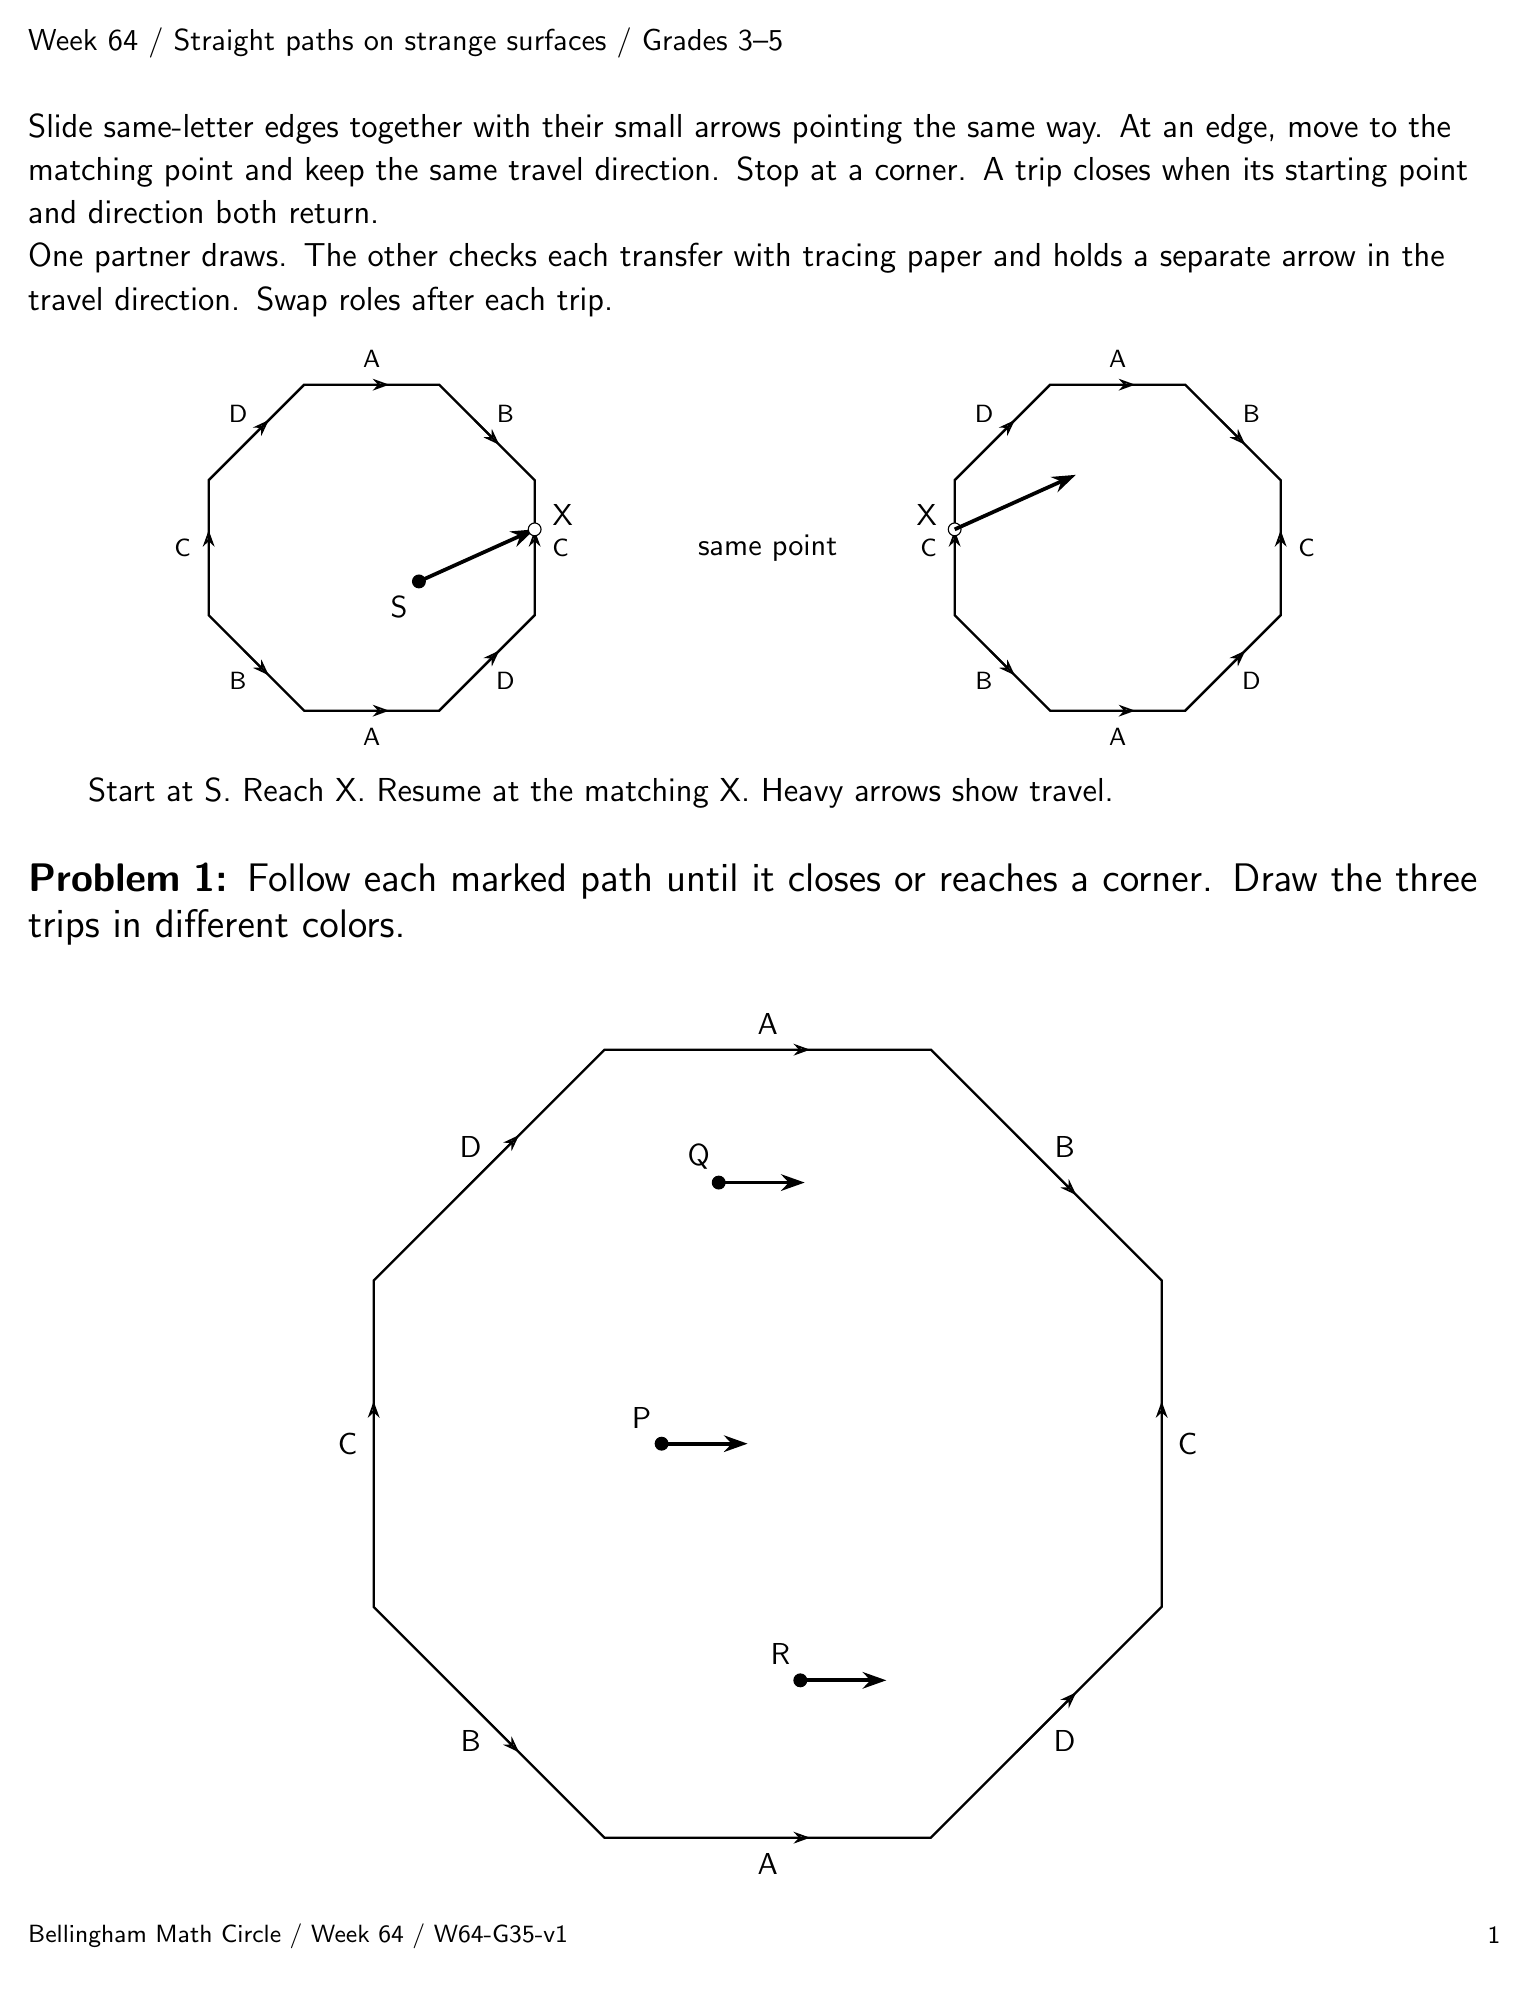
\begin{tikzpicture}[x=1in,y=-1in]
\path[use as bounding box] (0,0) rectangle (7.4,9.68);
\node[anchor=north west,inner sep=0pt,align=left,text width=7.4in,font=\fontsize{10.6}{13.25}\selectfont] at (0.00000,0.00000) {Week 64 / Straight paths on strange surfaces / Grades 3--5};
\node[anchor=north west,inner sep=0pt,align=left,text width=6.8in,font=\fontsize{9.5}{11.88}\selectfont] at (0.00000,9.48000) {Bellingham Math Circle / Week 64 / W64-G35-v1};
\node[anchor=east,inner sep=1pt,font=\fontsize{9.5}{10.5}\selectfont] at (7.38000,9.54000) {1};
\node[anchor=north west,inner sep=0pt,align=left,text width=7.35in,font=\fontsize{12.5}{15.62}\selectfont] at (0.00000,0.43000) {Slide same-letter edges together with their small arrows pointing the same way. At an edge, move to the matching point and keep the same travel direction. Stop at a corner. A trip closes when its starting point and direction both return.

One partner draws. The other checks each transfer with tracing paper and holds a separate arrow in the travel direction. Swap roles after each trip.};
\draw[line width=.85pt] (2.05758,1.78500) -- (2.53500,2.26242) -- (2.53500,2.93758) -- (2.05758,3.41500) -- (1.38242,3.41500) -- (0.90500,2.93758) -- (0.90500,2.26242) -- (1.38242,1.78500) -- cycle;
\draw[edge] (1.63223,1.78500) -- (1.80777,1.78500);
\node[anchor=center,inner sep=1pt,font=\fontsize{9}{10}\selectfont] at (1.72000,1.65500) {A};
\draw[edge] (2.23423,1.96164) -- (2.35836,2.08577);
\node[anchor=center,inner sep=1pt,font=\fontsize{9}{10}\selectfont] at (2.38822,1.93178) {B};
\draw[edge] (2.53500,2.68777) -- (2.53500,2.51223);
\node[anchor=center,inner sep=1pt,font=\fontsize{9}{10}\selectfont] at (2.66500,2.60000) {C};
\draw[edge] (2.23423,3.23836) -- (2.35836,3.11423);
\node[anchor=center,inner sep=1pt,font=\fontsize{9}{10}\selectfont] at (2.38822,3.26822) {D};
\draw[edge] (1.63223,3.41500) -- (1.80777,3.41500);
\node[anchor=center,inner sep=1pt,font=\fontsize{9}{10}\selectfont] at (1.72000,3.54500) {A};
\draw[edge] (1.08164,3.11423) -- (1.20577,3.23836);
\node[anchor=center,inner sep=1pt,font=\fontsize{9}{10}\selectfont] at (1.05178,3.26822) {B};
\draw[edge] (0.90500,2.68777) -- (0.90500,2.51223);
\node[anchor=center,inner sep=1pt,font=\fontsize{9}{10}\selectfont] at (0.77500,2.60000) {C};
\draw[edge] (1.08164,2.08577) -- (1.20577,1.96164);
\node[anchor=center,inner sep=1pt,font=\fontsize{9}{10}\selectfont] at (1.05178,1.93178) {D};
\draw[line width=.85pt] (5.78758,1.78500) -- (6.26500,2.26242) -- (6.26500,2.93758) -- (5.78758,3.41500) -- (5.11242,3.41500) -- (4.63500,2.93758) -- (4.63500,2.26242) -- (5.11242,1.78500) -- cycle;
\draw[edge] (5.36223,1.78500) -- (5.53777,1.78500);
\node[anchor=center,inner sep=1pt,font=\fontsize{9}{10}\selectfont] at (5.45000,1.65500) {A};
\draw[edge] (5.96423,1.96164) -- (6.08836,2.08577);
\node[anchor=center,inner sep=1pt,font=\fontsize{9}{10}\selectfont] at (6.11822,1.93178) {B};
\draw[edge] (6.26500,2.68777) -- (6.26500,2.51223);
\node[anchor=center,inner sep=1pt,font=\fontsize{9}{10}\selectfont] at (6.39500,2.60000) {C};
\draw[edge] (5.96423,3.23836) -- (6.08836,3.11423);
\node[anchor=center,inner sep=1pt,font=\fontsize{9}{10}\selectfont] at (6.11822,3.26822) {D};
\draw[edge] (5.36223,3.41500) -- (5.53777,3.41500);
\node[anchor=center,inner sep=1pt,font=\fontsize{9}{10}\selectfont] at (5.45000,3.54500) {A};
\draw[edge] (4.81164,3.11423) -- (4.93577,3.23836);
\node[anchor=center,inner sep=1pt,font=\fontsize{9}{10}\selectfont] at (4.78178,3.26822) {B};
\draw[edge] (4.63500,2.68777) -- (4.63500,2.51223);
\node[anchor=center,inner sep=1pt,font=\fontsize{9}{10}\selectfont] at (4.50500,2.60000) {C};
\draw[edge] (4.81164,2.08577) -- (4.93577,1.96164);
\node[anchor=center,inner sep=1pt,font=\fontsize{9}{10}\selectfont] at (4.78178,1.93178) {D};
\draw[fill=black] (1.95631,2.76879) circle[radius=.032in];
\node[anchor=center,inner sep=1pt,font=\fontsize{11}{12}\selectfont] at (1.85631,2.89879) {S};
\draw[travel] (1.95631,2.76879) -- (2.53500,2.50838);
\draw[fill=white] (2.53500,2.50838) circle[radius=.032in];
\node[anchor=center,inner sep=1pt,font=\fontsize{11}{12}\selectfont] at (2.67500,2.43838) {X};
\draw[fill=white] (4.63500,2.50838) circle[radius=.032in];
\node[anchor=center,inner sep=1pt,font=\fontsize{11}{12}\selectfont] at (4.49500,2.43838) {X};
\draw[travel] (4.63500,2.50838) -- (5.24070,2.23582);
\node[anchor=center,inner sep=1pt,font=\fontsize{11}{12}\selectfont] at (3.70000,2.60000) {same point};
\node[anchor=north west,inner sep=0pt,align=left,text width=6.8in,font=\fontsize{11.5}{14.38}\selectfont] at (0.30000,3.75000) {Start at S. Reach X. Resume at the matching X. Heavy arrows show travel.};
\node[anchor=north west,inner sep=0pt,align=left,text width=7.35in,font=\fontsize{13.3}{16.62}\selectfont] at (0.00000,4.18000) {\textbf{Problem 1:} Follow each marked path until it closes or reaches a corner. Draw the three trips in different colors.};
\draw[line width=.85pt] (4.51600,5.11000) -- (5.67000,6.26400) -- (5.67000,7.89600) -- (4.51600,9.05000) -- (2.88400,9.05000) -- (1.73000,7.89600) -- (1.73000,6.26400) -- (2.88400,5.11000) -- cycle;
\draw[edge] (3.48784,5.11000) -- (3.91216,5.11000);
\node[anchor=center,inner sep=1pt,font=\fontsize{11}{12}\selectfont] at (3.70000,4.98000) {A};
\draw[edge] (4.94298,5.53698) -- (5.24302,5.83702);
\node[anchor=center,inner sep=1pt,font=\fontsize{11}{12}\selectfont] at (5.18492,5.59508) {B};
\draw[edge] (5.67000,7.29216) -- (5.67000,6.86784);
\node[anchor=center,inner sep=1pt,font=\fontsize{11}{12}\selectfont] at (5.80000,7.08000) {C};
\draw[edge] (4.94298,8.62302) -- (5.24302,8.32298);
\node[anchor=center,inner sep=1pt,font=\fontsize{11}{12}\selectfont] at (5.18492,8.56492) {D};
\draw[edge] (3.48784,9.05000) -- (3.91216,9.05000);
\node[anchor=center,inner sep=1pt,font=\fontsize{11}{12}\selectfont] at (3.70000,9.18000) {A};
\draw[edge] (2.15698,8.32298) -- (2.45702,8.62302);
\node[anchor=center,inner sep=1pt,font=\fontsize{11}{12}\selectfont] at (2.21508,8.56492) {B};
\draw[edge] (1.73000,7.29216) -- (1.73000,6.86784);
\node[anchor=center,inner sep=1pt,font=\fontsize{11}{12}\selectfont] at (1.60000,7.08000) {C};
\draw[edge] (2.15698,5.83702) -- (2.45702,5.53698);
\node[anchor=center,inner sep=1pt,font=\fontsize{11}{12}\selectfont] at (2.21508,5.59508) {D};
\draw[fill=black] (3.16960,7.08000) circle[radius=.032in];
\node[anchor=center,inner sep=1pt,font=\fontsize{11}{12}\selectfont] at (3.06960,6.95000) {P};
\draw[travel] (3.16960,7.08000) -- (3.59960,7.08000);
\draw[fill=black] (3.45520,5.77440) circle[radius=.032in];
\node[anchor=center,inner sep=1pt,font=\fontsize{11}{12}\selectfont] at (3.35520,5.64440) {Q};
\draw[travel] (3.45520,5.77440) -- (3.88520,5.77440);
\draw[fill=black] (3.86320,8.26320) circle[radius=.032in];
\node[anchor=center,inner sep=1pt,font=\fontsize{11}{12}\selectfont] at (3.76320,8.13320) {R};
\draw[travel] (3.86320,8.26320) -- (4.29320,8.26320);
\end{tikzpicture}\newpage
\noindent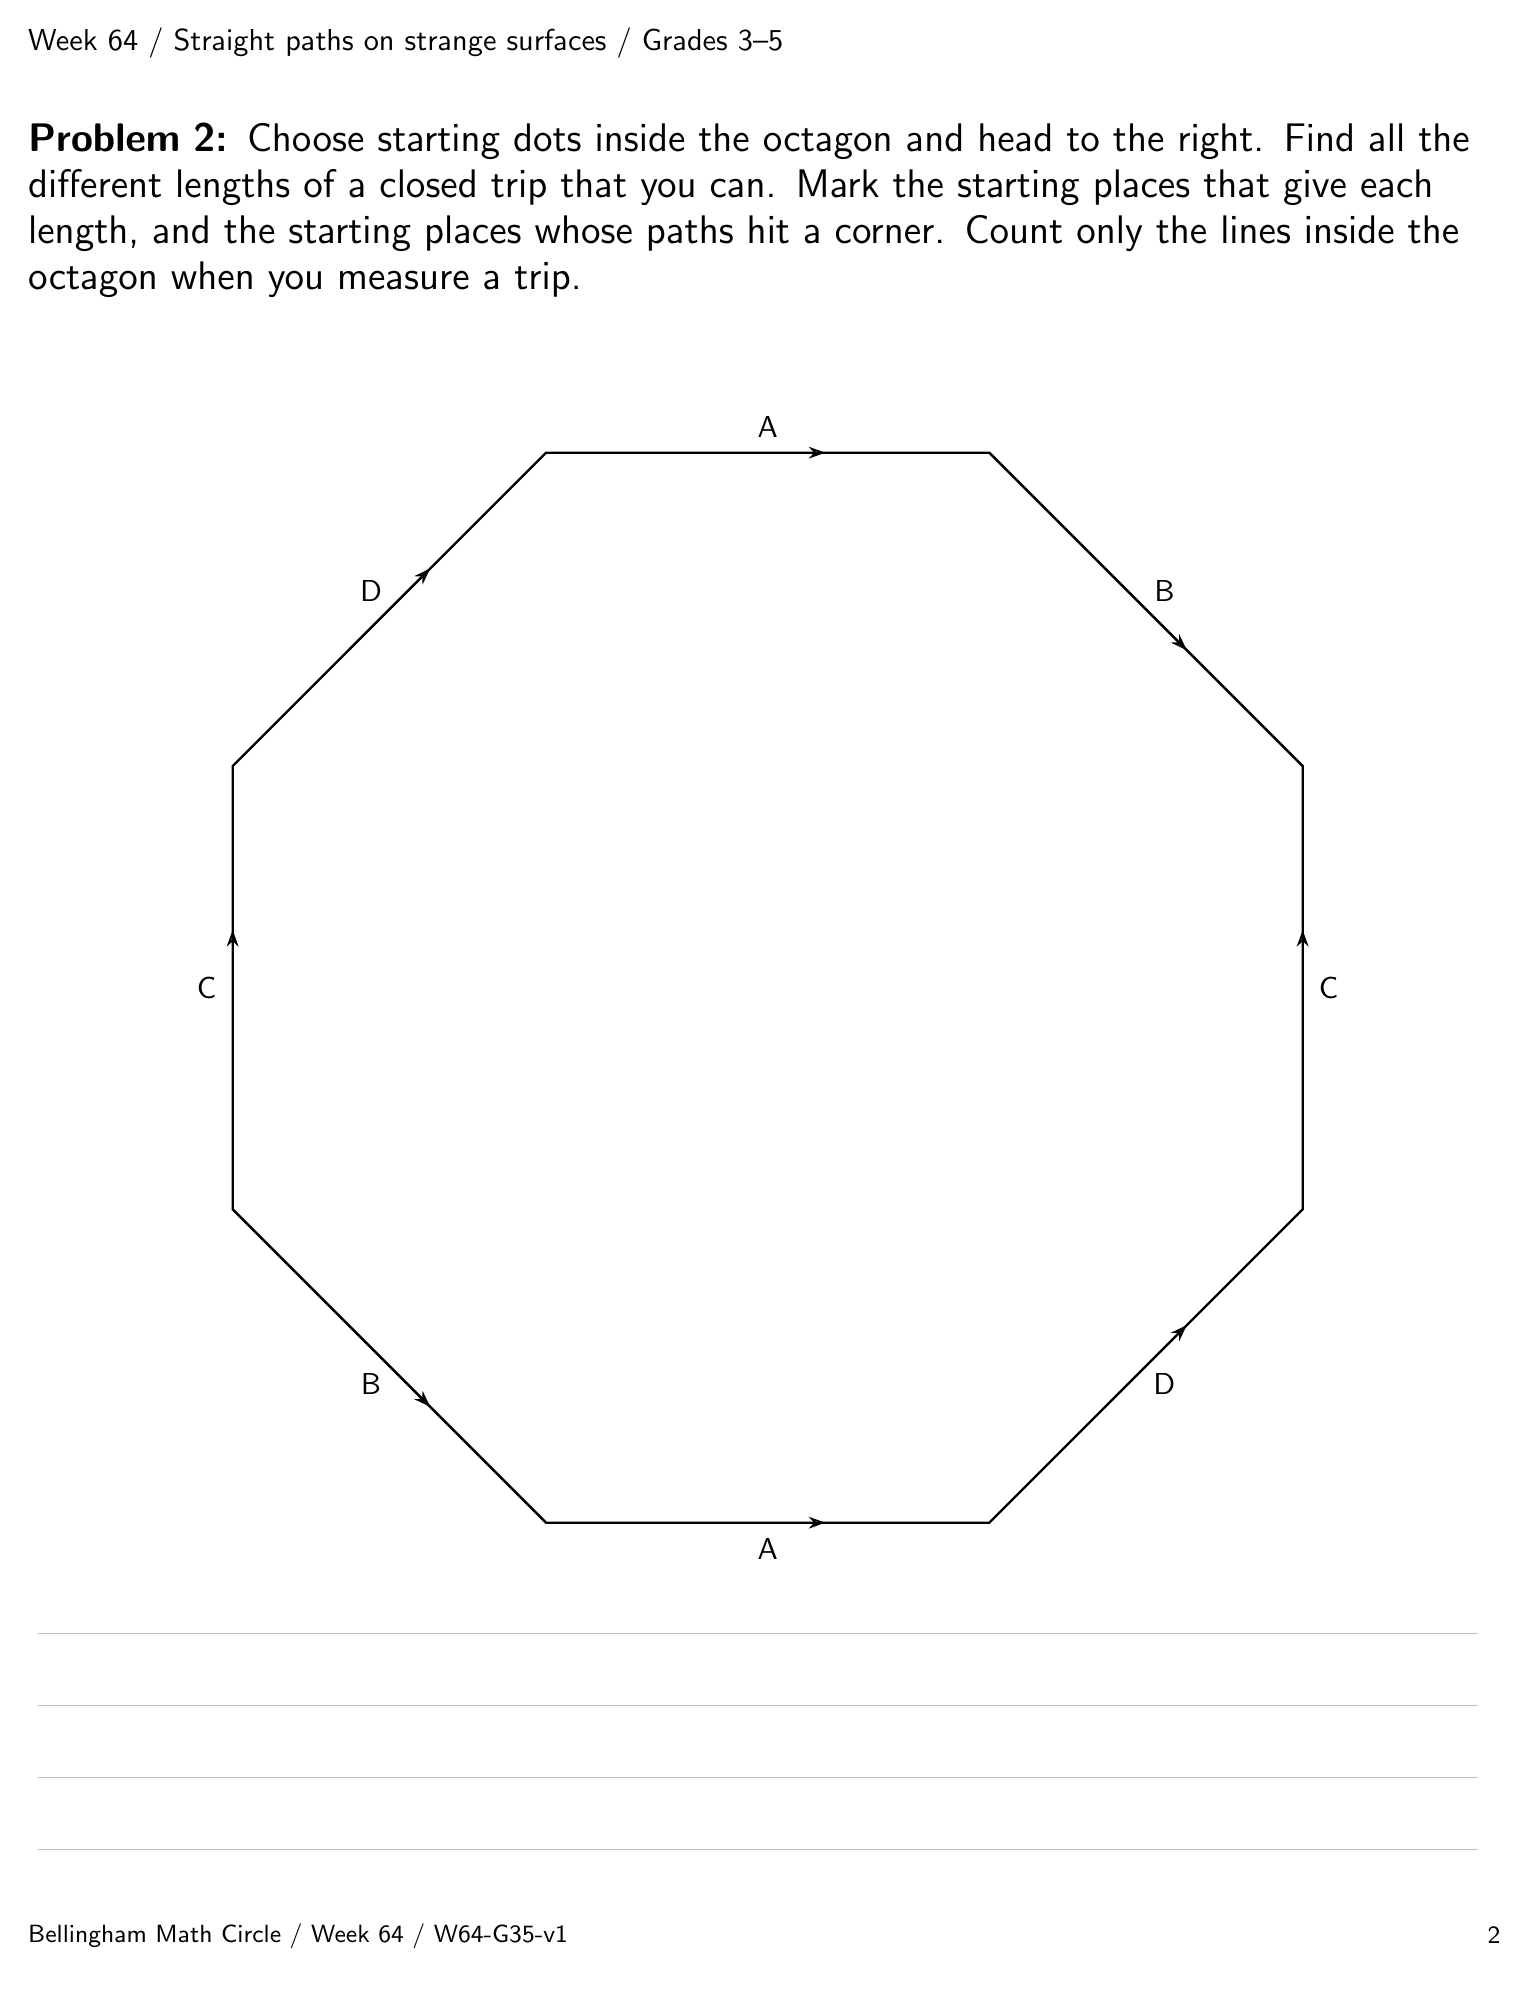
\begin{tikzpicture}[x=1in,y=-1in]
\path[use as bounding box] (0,0) rectangle (7.4,9.68);
\node[anchor=north west,inner sep=0pt,align=left,text width=7.4in,font=\fontsize{10.6}{13.25}\selectfont] at (0.00000,0.00000) {Week 64 / Straight paths on strange surfaces / Grades 3--5};
\node[anchor=north west,inner sep=0pt,align=left,text width=6.8in,font=\fontsize{9.5}{11.88}\selectfont] at (0.00000,9.48000) {Bellingham Math Circle / Week 64 / W64-G35-v1};
\node[anchor=east,inner sep=1pt,font=\fontsize{9.5}{10.5}\selectfont] at (7.38000,9.54000) {2};
\node[anchor=north west,inner sep=0pt,align=left,text width=7.35in,font=\fontsize{13.3}{16.62}\selectfont] at (0.00000,0.48000) {\textbf{Problem 2:} Choose starting dots inside the octagon and head to the right. Find all the different lengths of a closed trip that you can. Mark the starting places that give each length, and the starting places whose paths hit a corner. Count only the lines inside the octagon when you measure a trip.};
\draw[line width=.85pt] (4.80802,2.12500) -- (6.37500,3.69198) -- (6.37500,5.90802) -- (4.80802,7.47500) -- (2.59198,7.47500) -- (1.02500,5.90802) -- (1.02500,3.69198) -- (2.59198,2.12500) -- cycle;
\draw[edge] (3.41191,2.12500) -- (3.98809,2.12500);
\node[anchor=center,inner sep=1pt,font=\fontsize{11}{12}\selectfont] at (3.70000,1.99500) {A};
\draw[edge] (5.38780,2.70478) -- (5.79522,3.11220);
\node[anchor=center,inner sep=1pt,font=\fontsize{11}{12}\selectfont] at (5.68343,2.81657) {B};
\draw[edge] (6.37500,5.08809) -- (6.37500,4.51191);
\node[anchor=center,inner sep=1pt,font=\fontsize{11}{12}\selectfont] at (6.50500,4.80000) {C};
\draw[edge] (5.38780,6.89522) -- (5.79522,6.48780);
\node[anchor=center,inner sep=1pt,font=\fontsize{11}{12}\selectfont] at (5.68343,6.78343) {D};
\draw[edge] (3.41191,7.47500) -- (3.98809,7.47500);
\node[anchor=center,inner sep=1pt,font=\fontsize{11}{12}\selectfont] at (3.70000,7.60500) {A};
\draw[edge] (1.60478,6.48780) -- (2.01220,6.89522);
\node[anchor=center,inner sep=1pt,font=\fontsize{11}{12}\selectfont] at (1.71657,6.78343) {B};
\draw[edge] (1.02500,5.08809) -- (1.02500,4.51191);
\node[anchor=center,inner sep=1pt,font=\fontsize{11}{12}\selectfont] at (0.89500,4.80000) {C};
\draw[edge] (1.60478,3.11220) -- (2.01220,2.70478);
\node[anchor=center,inner sep=1pt,font=\fontsize{11}{12}\selectfont] at (1.71657,2.81657) {D};
\draw[black!25,line width=.35pt] (0.05000,8.03000) -- (7.25000,8.03000);
\draw[black!25,line width=.35pt] (0.05000,8.39000) -- (7.25000,8.39000);
\draw[black!25,line width=.35pt] (0.05000,8.75000) -- (7.25000,8.75000);
\draw[black!25,line width=.35pt] (0.05000,9.11000) -- (7.25000,9.11000);
\end{tikzpicture}\newpage
\noindent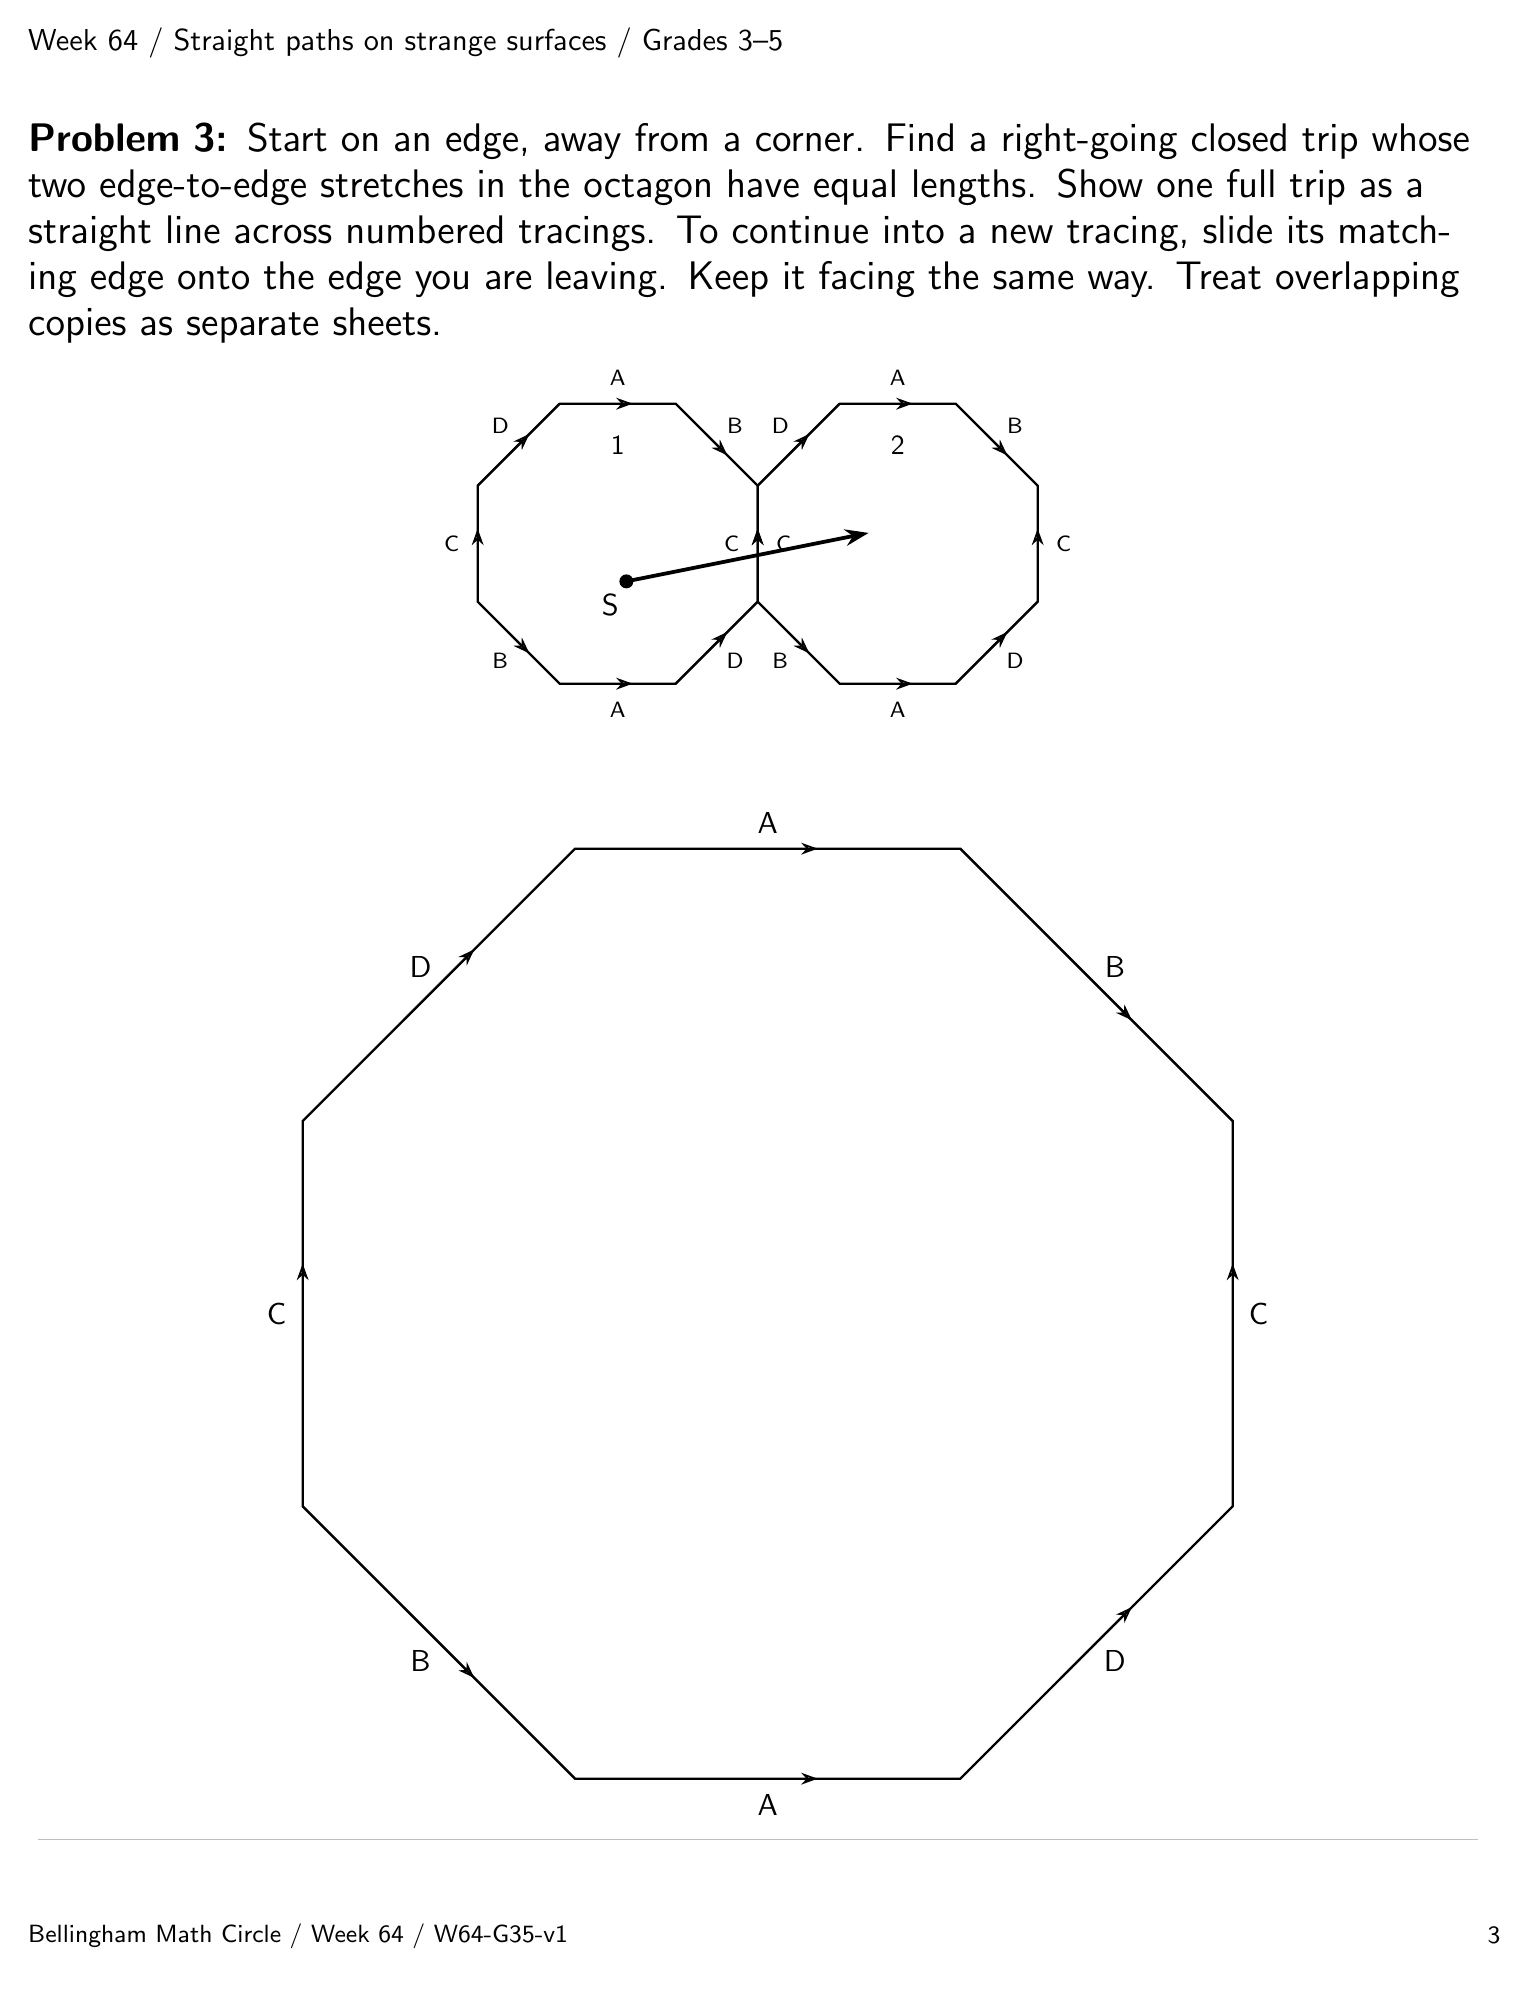
\begin{tikzpicture}[x=1in,y=-1in]
\path[use as bounding box] (0,0) rectangle (7.4,9.68);
\node[anchor=north west,inner sep=0pt,align=left,text width=7.4in,font=\fontsize{10.6}{13.25}\selectfont] at (0.00000,0.00000) {Week 64 / Straight paths on strange surfaces / Grades 3--5};
\node[anchor=north west,inner sep=0pt,align=left,text width=6.8in,font=\fontsize{9.5}{11.88}\selectfont] at (0.00000,9.48000) {Bellingham Math Circle / Week 64 / W64-G35-v1};
\node[anchor=east,inner sep=1pt,font=\fontsize{9.5}{10.5}\selectfont] at (7.38000,9.54000) {3};
\node[anchor=north west,inner sep=0pt,align=left,text width=7.35in,font=\fontsize{13.3}{16.62}\selectfont] at (0.00000,0.48000) {\textbf{Problem 3:} Start on an edge, away from a corner. Find a right-going closed trip whose two edge-to-edge stretches in the octagon have equal lengths. Show one full trip as a straight line across numbered tracings. To continue into a new tracing, slide its matching edge onto the edge you are leaving. Keep it facing the same way. Treat overlapping copies as separate sheets.};
\draw[line width=.85pt] (3.23995,1.88000) -- (3.65000,2.29005) -- (3.65000,2.86995) -- (3.23995,3.28000) -- (2.66005,3.28000) -- (2.25000,2.86995) -- (2.25000,2.29005) -- (2.66005,1.88000) -- cycle;
\draw[edge] (2.87461,1.88000) -- (3.02539,1.88000);
\node[anchor=center,inner sep=1pt,font=\fontsize{8}{9}\selectfont] at (2.95000,1.75000) {A};
\draw[edge] (3.39167,2.03172) -- (3.49828,2.13833);
\node[anchor=center,inner sep=1pt,font=\fontsize{8}{9}\selectfont] at (3.53690,1.99310) {B};
\draw[edge] (3.65000,2.65539) -- (3.65000,2.50461);
\node[anchor=center,inner sep=1pt,font=\fontsize{8}{9}\selectfont] at (3.78000,2.58000) {C};
\draw[edge] (3.39167,3.12828) -- (3.49828,3.02167);
\node[anchor=center,inner sep=1pt,font=\fontsize{8}{9}\selectfont] at (3.53690,3.16690) {D};
\draw[edge] (2.87461,3.28000) -- (3.02539,3.28000);
\node[anchor=center,inner sep=1pt,font=\fontsize{8}{9}\selectfont] at (2.95000,3.41000) {A};
\draw[edge] (2.40172,3.02167) -- (2.50833,3.12828);
\node[anchor=center,inner sep=1pt,font=\fontsize{8}{9}\selectfont] at (2.36310,3.16690) {B};
\draw[edge] (2.25000,2.65539) -- (2.25000,2.50461);
\node[anchor=center,inner sep=1pt,font=\fontsize{8}{9}\selectfont] at (2.12000,2.58000) {C};
\draw[edge] (2.40172,2.13833) -- (2.50833,2.03172);
\node[anchor=center,inner sep=1pt,font=\fontsize{8}{9}\selectfont] at (2.36310,1.99310) {D};
\draw[line width=.85pt] (4.63995,1.88000) -- (5.05000,2.29005) -- (5.05000,2.86995) -- (4.63995,3.28000) -- (4.06005,3.28000) -- (3.65000,2.86995) -- (3.65000,2.29005) -- (4.06005,1.88000) -- cycle;
\draw[edge] (4.27461,1.88000) -- (4.42539,1.88000);
\node[anchor=center,inner sep=1pt,font=\fontsize{8}{9}\selectfont] at (4.35000,1.75000) {A};
\draw[edge] (4.79167,2.03172) -- (4.89828,2.13833);
\node[anchor=center,inner sep=1pt,font=\fontsize{8}{9}\selectfont] at (4.93690,1.99310) {B};
\draw[edge] (5.05000,2.65539) -- (5.05000,2.50461);
\node[anchor=center,inner sep=1pt,font=\fontsize{8}{9}\selectfont] at (5.18000,2.58000) {C};
\draw[edge] (4.79167,3.12828) -- (4.89828,3.02167);
\node[anchor=center,inner sep=1pt,font=\fontsize{8}{9}\selectfont] at (4.93690,3.16690) {D};
\draw[edge] (4.27461,3.28000) -- (4.42539,3.28000);
\node[anchor=center,inner sep=1pt,font=\fontsize{8}{9}\selectfont] at (4.35000,3.41000) {A};
\draw[edge] (3.80172,3.02167) -- (3.90833,3.12828);
\node[anchor=center,inner sep=1pt,font=\fontsize{8}{9}\selectfont] at (3.76310,3.16690) {B};
\draw[edge] (3.65000,2.65539) -- (3.65000,2.50461);
\node[anchor=center,inner sep=1pt,font=\fontsize{8}{9}\selectfont] at (3.52000,2.58000) {C};
\draw[edge] (3.80172,2.13833) -- (3.90833,2.03172);
\node[anchor=center,inner sep=1pt,font=\fontsize{8}{9}\selectfont] at (3.76310,1.99310) {D};
\draw[fill=black] (2.99349,2.76847) circle[radius=.032in];
\node[anchor=center,inner sep=1pt,font=\fontsize{11}{12}\selectfont] at (2.91349,2.88847) {S};
\draw[line width=1.35pt] (2.99349,2.76847) -- (3.65000,2.63717);
\draw[travel] (3.65000,2.63717) -- (4.20503,2.52616);
\node[anchor=center,inner sep=1pt,font=\fontsize{10}{11}\selectfont] at (2.95000,2.09000) {1};
\node[anchor=center,inner sep=1pt,font=\fontsize{10}{11}\selectfont] at (4.35000,2.09000) {2};
\draw[line width=.85pt] (4.66305,4.10500) -- (6.02500,5.46695) -- (6.02500,7.39305) -- (4.66305,8.75500) -- (2.73695,8.75500) -- (1.37500,7.39305) -- (1.37500,5.46695) -- (2.73695,4.10500) -- cycle;
\draw[edge] (3.44961,4.10500) -- (3.95039,4.10500);
\node[anchor=center,inner sep=1pt,font=\fontsize{11}{12}\selectfont] at (3.70000,3.97500) {A};
\draw[edge] (5.16697,4.60892) -- (5.52108,4.96303);
\node[anchor=center,inner sep=1pt,font=\fontsize{11}{12}\selectfont] at (5.43595,4.69405) {B};
\draw[edge] (6.02500,6.68039) -- (6.02500,6.17961);
\node[anchor=center,inner sep=1pt,font=\fontsize{11}{12}\selectfont] at (6.15500,6.43000) {C};
\draw[edge] (5.16697,8.25108) -- (5.52108,7.89697);
\node[anchor=center,inner sep=1pt,font=\fontsize{11}{12}\selectfont] at (5.43595,8.16595) {D};
\draw[edge] (3.44961,8.75500) -- (3.95039,8.75500);
\node[anchor=center,inner sep=1pt,font=\fontsize{11}{12}\selectfont] at (3.70000,8.88500) {A};
\draw[edge] (1.87892,7.89697) -- (2.23303,8.25108);
\node[anchor=center,inner sep=1pt,font=\fontsize{11}{12}\selectfont] at (1.96405,8.16595) {B};
\draw[edge] (1.37500,6.68039) -- (1.37500,6.17961);
\node[anchor=center,inner sep=1pt,font=\fontsize{11}{12}\selectfont] at (1.24500,6.43000) {C};
\draw[edge] (1.87892,4.96303) -- (2.23303,4.60892);
\node[anchor=center,inner sep=1pt,font=\fontsize{11}{12}\selectfont] at (1.96405,4.69405) {D};
\draw[black!25,line width=.35pt] (0.05000,9.06000) -- (7.25000,9.06000);
\end{tikzpicture}\newpage
\noindent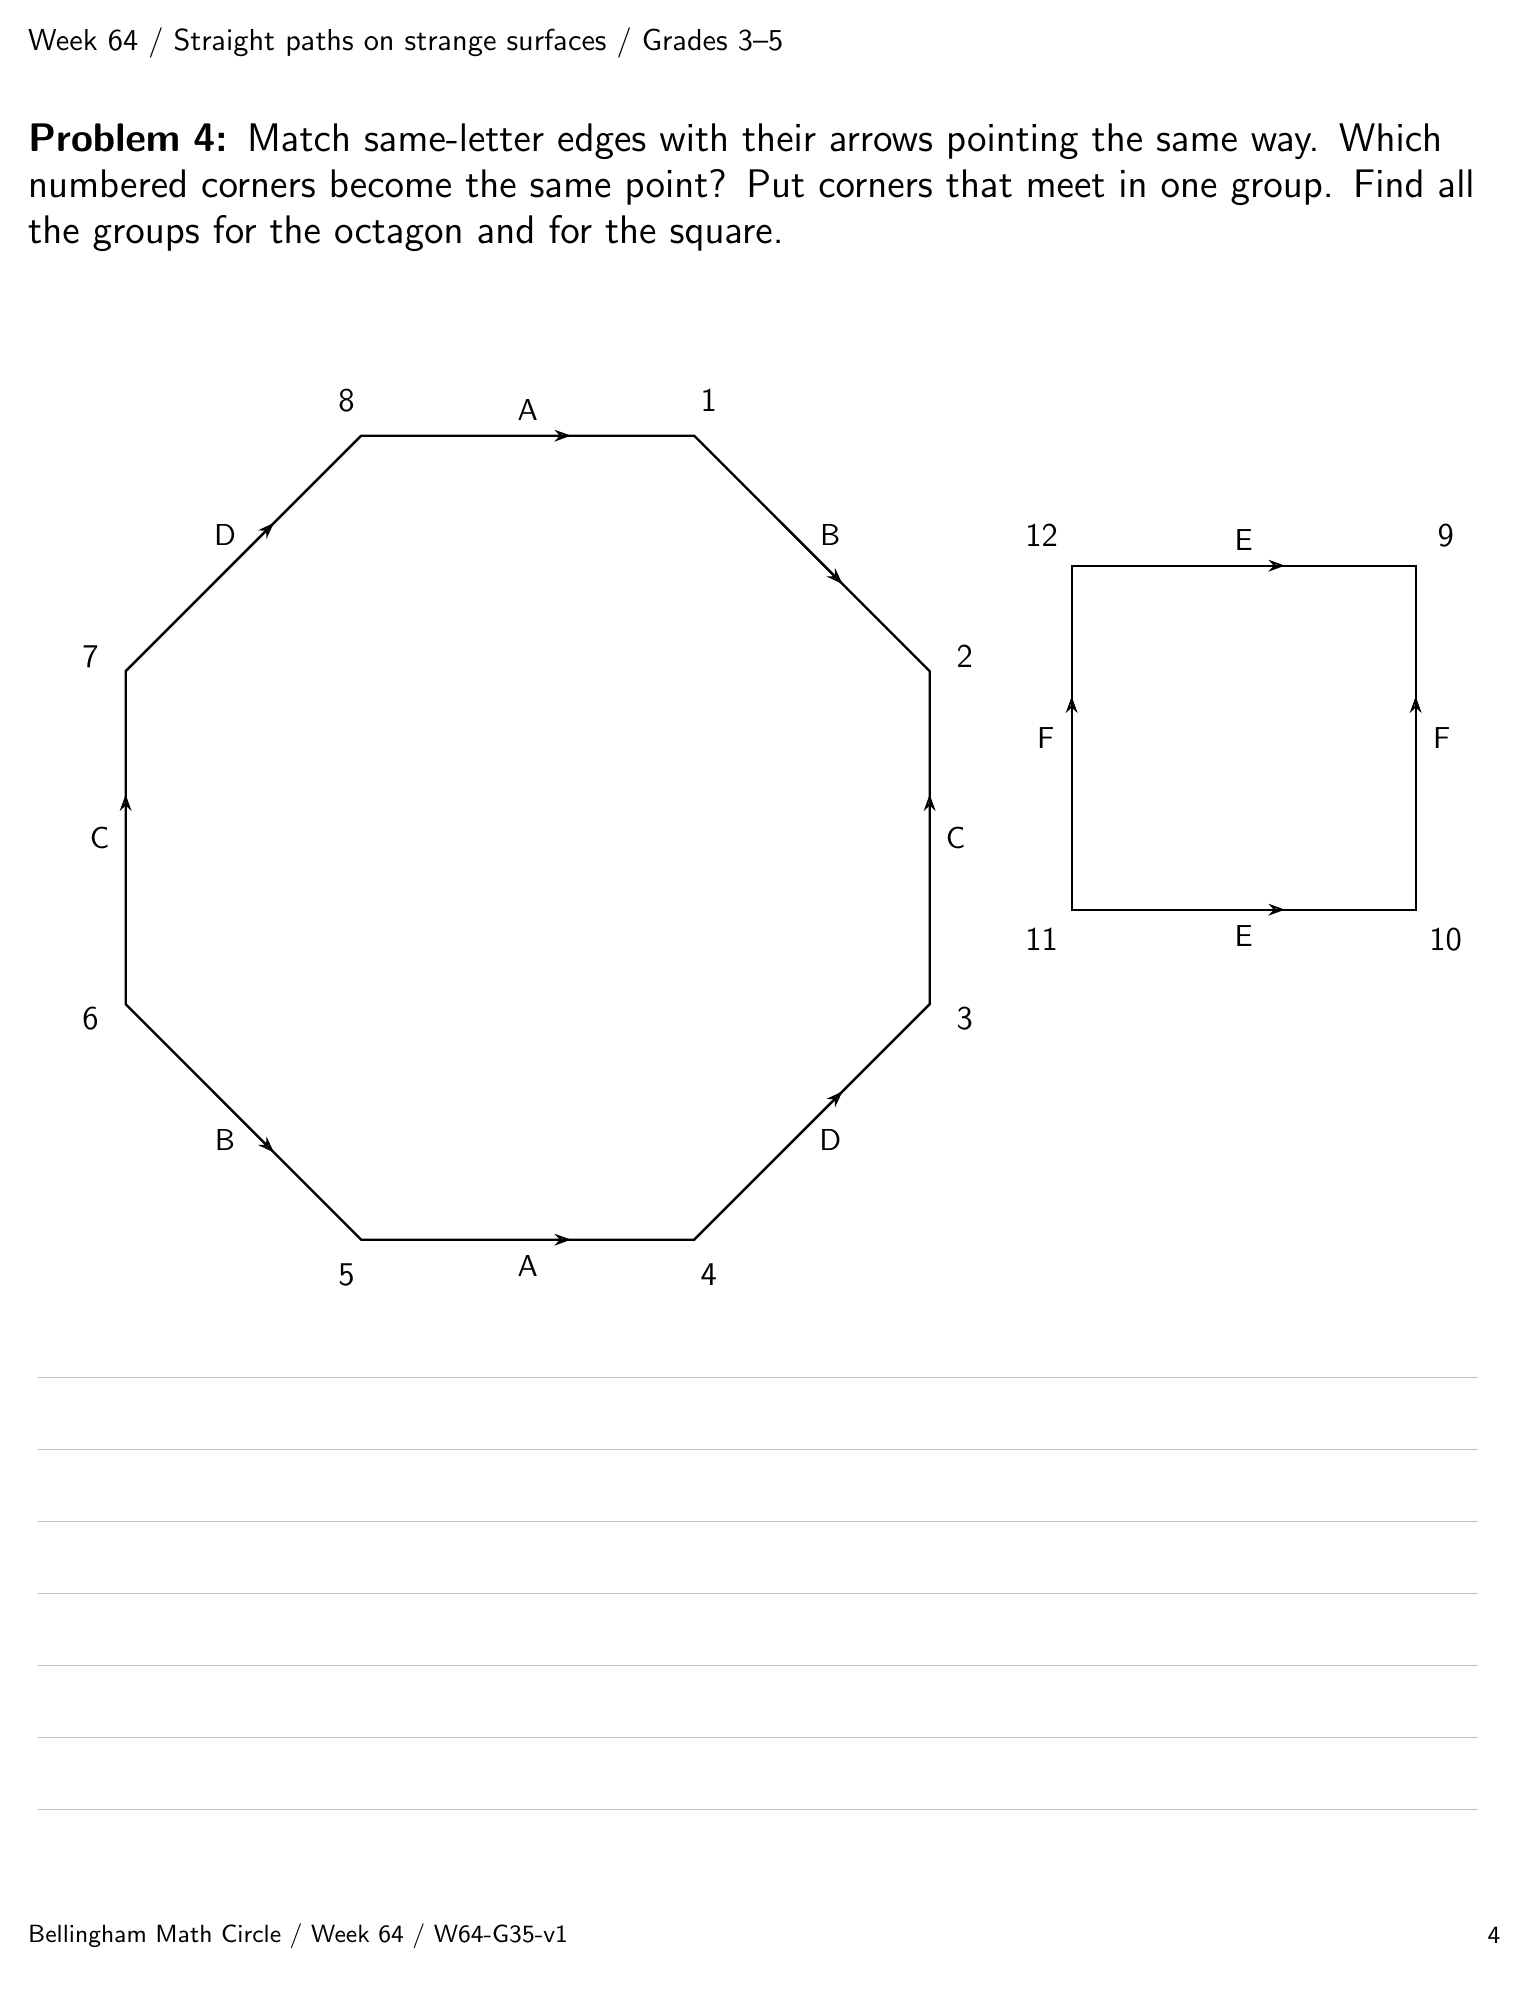
\begin{tikzpicture}[x=1in,y=-1in]
\path[use as bounding box] (0,0) rectangle (7.4,9.68);
\node[anchor=north west,inner sep=0pt,align=left,text width=7.4in,font=\fontsize{10.6}{13.25}\selectfont] at (0.00000,0.00000) {Week 64 / Straight paths on strange surfaces / Grades 3--5};
\node[anchor=north west,inner sep=0pt,align=left,text width=6.8in,font=\fontsize{9.5}{11.88}\selectfont] at (0.00000,9.48000) {Bellingham Math Circle / Week 64 / W64-G35-v1};
\node[anchor=east,inner sep=1pt,font=\fontsize{9.5}{10.5}\selectfont] at (7.38000,9.54000) {4};
\node[anchor=north west,inner sep=0pt,align=left,text width=7.35in,font=\fontsize{13.3}{16.62}\selectfont] at (0.00000,0.48000) {\textbf{Problem 4:} Match same-letter edges with their arrows pointing the same way. Which numbered corners become the same point? Put corners that meet in one group. Find all the groups for the octagon and for the square.};
\draw[line width=.85pt] (3.33257,2.04000) -- (4.51000,3.21743) -- (4.51000,4.88257) -- (3.33257,6.06000) -- (1.66743,6.06000) -- (0.49000,4.88257) -- (0.49000,3.21743) -- (1.66743,2.04000) -- cycle;
\draw[edge] (2.28353,2.04000) -- (2.71647,2.04000);
\node[anchor=center,inner sep=1pt,font=\fontsize{11}{12}\selectfont] at (2.50000,1.91000) {A};
\draw[edge] (3.76822,2.47565) -- (4.07435,2.78178);
\node[anchor=center,inner sep=1pt,font=\fontsize{11}{12}\selectfont] at (4.01321,2.53679) {B};
\draw[edge] (4.51000,4.26647) -- (4.51000,3.83353);
\node[anchor=center,inner sep=1pt,font=\fontsize{11}{12}\selectfont] at (4.64000,4.05000) {C};
\draw[edge] (3.76822,5.62435) -- (4.07435,5.31822);
\node[anchor=center,inner sep=1pt,font=\fontsize{11}{12}\selectfont] at (4.01321,5.56321) {D};
\draw[edge] (2.28353,6.06000) -- (2.71647,6.06000);
\node[anchor=center,inner sep=1pt,font=\fontsize{11}{12}\selectfont] at (2.50000,6.19000) {A};
\draw[edge] (0.92565,5.31822) -- (1.23178,5.62435);
\node[anchor=center,inner sep=1pt,font=\fontsize{11}{12}\selectfont] at (0.98679,5.56321) {B};
\draw[edge] (0.49000,4.26647) -- (0.49000,3.83353);
\node[anchor=center,inner sep=1pt,font=\fontsize{11}{12}\selectfont] at (0.36000,4.05000) {C};
\draw[edge] (0.92565,2.78178) -- (1.23178,2.47565);
\node[anchor=center,inner sep=1pt,font=\fontsize{11}{12}\selectfont] at (0.98679,2.53679) {D};
\node[anchor=center,inner sep=1pt,font=\fontsize{12}{13}\selectfont] at (3.40528,1.86446) {1};
\node[anchor=center,inner sep=1pt,font=\fontsize{12}{13}\selectfont] at (4.68554,3.14472) {2};
\node[anchor=center,inner sep=1pt,font=\fontsize{12}{13}\selectfont] at (4.68554,4.95528) {3};
\node[anchor=center,inner sep=1pt,font=\fontsize{12}{13}\selectfont] at (3.40528,6.23554) {4};
\node[anchor=center,inner sep=1pt,font=\fontsize{12}{13}\selectfont] at (1.59472,6.23554) {5};
\node[anchor=center,inner sep=1pt,font=\fontsize{12}{13}\selectfont] at (0.31446,4.95528) {6};
\node[anchor=center,inner sep=1pt,font=\fontsize{12}{13}\selectfont] at (0.31446,3.14472) {7};
\node[anchor=center,inner sep=1pt,font=\fontsize{12}{13}\selectfont] at (1.59472,1.86446) {8};
\draw[line width=.85pt] (6.94000,2.69000) -- (6.94000,4.41000) -- (5.22000,4.41000) -- (5.22000,2.69000) -- cycle;
\draw[edge] (5.87360,2.69000) -- (6.28640,2.69000);
\node[anchor=center,inner sep=1pt,font=\fontsize{11}{12}\selectfont] at (6.08000,2.56000) {E};
\draw[edge] (6.94000,3.75640) -- (6.94000,3.34360);
\node[anchor=center,inner sep=1pt,font=\fontsize{11}{12}\selectfont] at (7.07000,3.55000) {F};
\draw[edge] (5.87360,4.41000) -- (6.28640,4.41000);
\node[anchor=center,inner sep=1pt,font=\fontsize{11}{12}\selectfont] at (6.08000,4.54000) {E};
\draw[edge] (5.22000,3.75640) -- (5.22000,3.34360);
\node[anchor=center,inner sep=1pt,font=\fontsize{11}{12}\selectfont] at (5.09000,3.55000) {F};
\node[anchor=center,inner sep=1pt,font=\fontsize{12}{13}\selectfont] at (7.09000,2.54000) {9};
\node[anchor=center,inner sep=1pt,font=\fontsize{12}{13}\selectfont] at (7.09000,4.56000) {10};
\node[anchor=center,inner sep=1pt,font=\fontsize{12}{13}\selectfont] at (5.07000,4.56000) {11};
\node[anchor=center,inner sep=1pt,font=\fontsize{12}{13}\selectfont] at (5.07000,2.54000) {12};
\draw[black!25,line width=.35pt] (0.05000,6.75000) -- (7.25000,6.75000);
\draw[black!25,line width=.35pt] (0.05000,7.11000) -- (7.25000,7.11000);
\draw[black!25,line width=.35pt] (0.05000,7.47000) -- (7.25000,7.47000);
\draw[black!25,line width=.35pt] (0.05000,7.83000) -- (7.25000,7.83000);
\draw[black!25,line width=.35pt] (0.05000,8.19000) -- (7.25000,8.19000);
\draw[black!25,line width=.35pt] (0.05000,8.55000) -- (7.25000,8.55000);
\draw[black!25,line width=.35pt] (0.05000,8.91000) -- (7.25000,8.91000);
\end{tikzpicture}\newpage
\noindent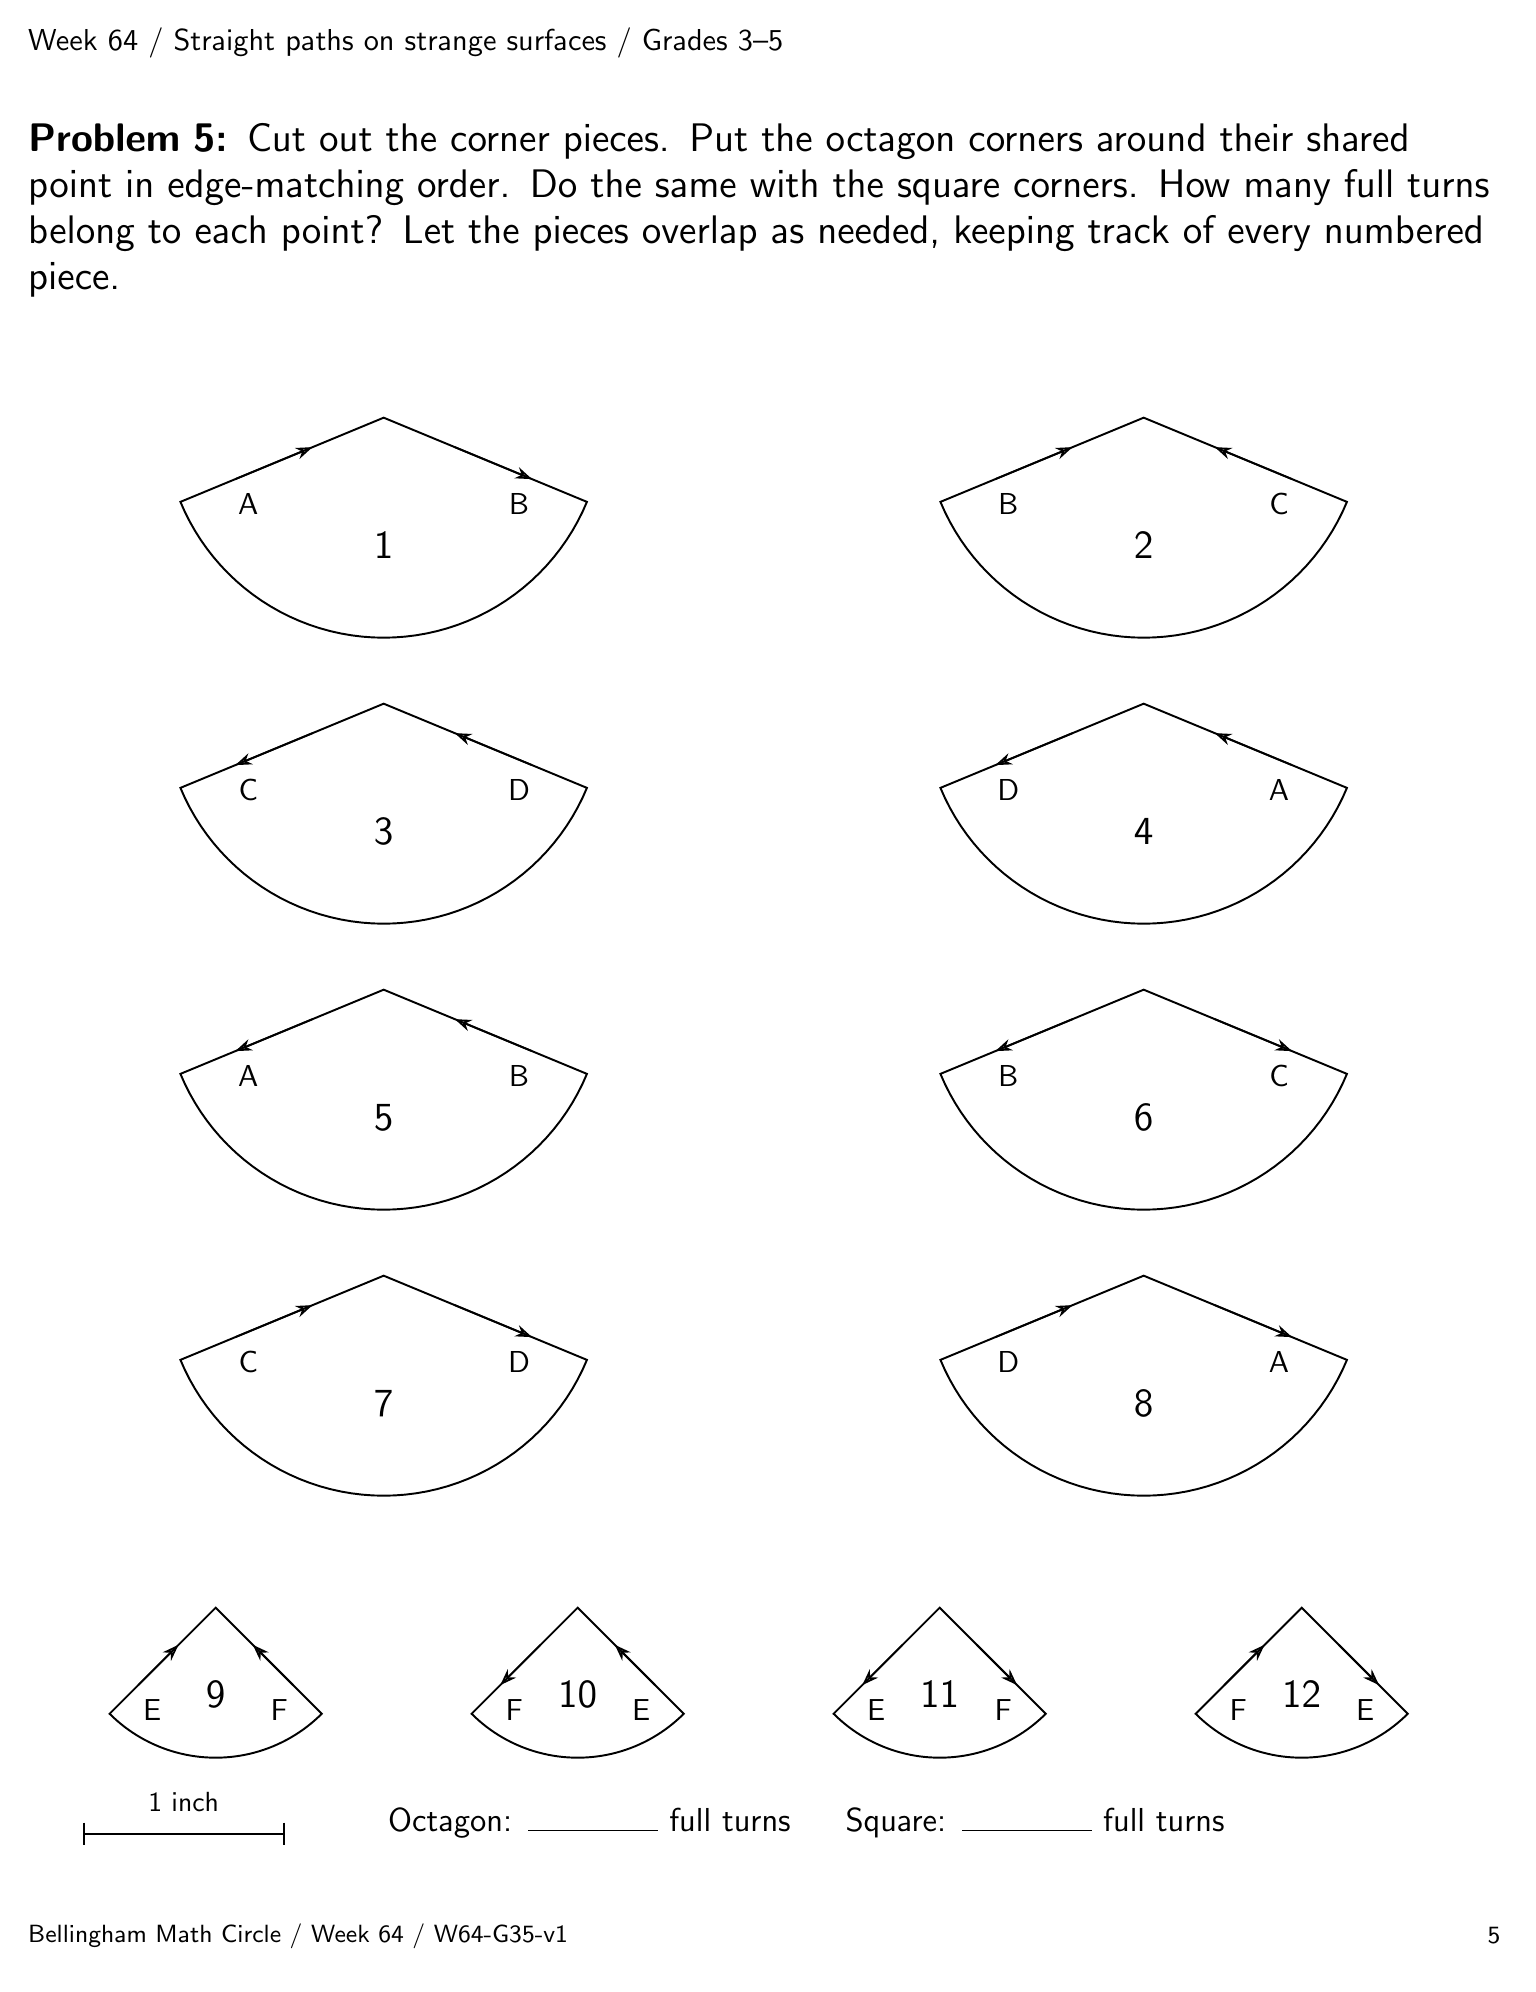
\begin{tikzpicture}[x=1in,y=-1in]
\path[use as bounding box] (0,0) rectangle (7.4,9.68);
\node[anchor=north west,inner sep=0pt,align=left,text width=7.4in,font=\fontsize{10.6}{13.25}\selectfont] at (0.00000,0.00000) {Week 64 / Straight paths on strange surfaces / Grades 3--5};
\node[anchor=north west,inner sep=0pt,align=left,text width=6.8in,font=\fontsize{9.5}{11.88}\selectfont] at (0.00000,9.48000) {Bellingham Math Circle / Week 64 / W64-G35-v1};
\node[anchor=east,inner sep=1pt,font=\fontsize{9.5}{10.5}\selectfont] at (7.38000,9.54000) {5};
\node[anchor=north west,inner sep=0pt,align=left,text width=7.35in,font=\fontsize{13.3}{16.62}\selectfont] at (0.00000,0.48000) {\textbf{Problem 5:} Cut out the corner pieces. Put the octagon corners around their shared point in edge-matching order. Do the same with the square corners. How many full turns belong to each point? Let the pieces overlap as needed, keeping track of every numbered piece.};
\draw[line width=.7pt] (1.78000,1.95000) -- (0.76373,2.37095) -- (0.78561,2.42031) -- (0.80989,2.46854) -- (0.83650,2.51551) -- (0.86538,2.56113) -- (0.89647,2.60527) -- (0.92969,2.64783) -- (0.96495,2.68871) -- (1.00218,2.72782) -- (1.04129,2.76505) -- (1.08217,2.80031) -- (1.12473,2.83353) -- (1.16887,2.86462) -- (1.21449,2.89350) -- (1.26146,2.92011) -- (1.30969,2.94439) -- (1.35905,2.96627) -- (1.40942,2.98570) -- (1.46069,3.00263) -- (1.51272,3.01703) -- (1.56540,3.02886) -- (1.61860,3.03809) -- (1.67218,3.04470) -- (1.72603,3.04868) -- (1.78000,3.05000) -- (1.83397,3.04868) -- (1.88782,3.04470) -- (1.94140,3.03809) -- (1.99460,3.02886) -- (2.04728,3.01703) -- (2.09931,3.00263) -- (2.15058,2.98570) -- (2.20095,2.96627) -- (2.25031,2.94439) -- (2.29854,2.92011) -- (2.34551,2.89350) -- (2.39113,2.86462) -- (2.43527,2.83353) -- (2.47783,2.80031) -- (2.51871,2.76505) -- (2.55782,2.72782) -- (2.59505,2.68871) -- (2.63031,2.64783) -- (2.66353,2.60527) -- (2.69462,2.56113) -- (2.72350,2.51551) -- (2.75011,2.46854) -- (2.77439,2.42031) -- (2.79627,2.37095) -- cycle;
\draw[edge] (1.03812,2.25729) -- (1.42431,2.09733);
\node[anchor=center,inner sep=1pt,font=\fontsize{11}{12}\selectfont] at (1.10296,2.38150) {A};
\draw[edge] (2.13569,2.09733) -- (2.52188,2.25729);
\node[anchor=center,inner sep=1pt,font=\fontsize{11}{12}\selectfont] at (2.45704,2.38150) {B};
\node[anchor=center,inner sep=1pt,font=\fontsize{14}{15}\selectfont] at (1.78000,2.58800) {1};
\draw[line width=.7pt] (5.58000,1.95000) -- (4.56373,2.37095) -- (4.58561,2.42031) -- (4.60989,2.46854) -- (4.63650,2.51551) -- (4.66538,2.56113) -- (4.69647,2.60527) -- (4.72969,2.64783) -- (4.76495,2.68871) -- (4.80218,2.72782) -- (4.84129,2.76505) -- (4.88217,2.80031) -- (4.92473,2.83353) -- (4.96887,2.86462) -- (5.01449,2.89350) -- (5.06146,2.92011) -- (5.10969,2.94439) -- (5.15905,2.96627) -- (5.20942,2.98570) -- (5.26069,3.00263) -- (5.31272,3.01703) -- (5.36540,3.02886) -- (5.41860,3.03809) -- (5.47218,3.04470) -- (5.52603,3.04868) -- (5.58000,3.05000) -- (5.63397,3.04868) -- (5.68782,3.04470) -- (5.74140,3.03809) -- (5.79460,3.02886) -- (5.84728,3.01703) -- (5.89931,3.00263) -- (5.95058,2.98570) -- (6.00095,2.96627) -- (6.05031,2.94439) -- (6.09854,2.92011) -- (6.14551,2.89350) -- (6.19113,2.86462) -- (6.23527,2.83353) -- (6.27783,2.80031) -- (6.31871,2.76505) -- (6.35782,2.72782) -- (6.39505,2.68871) -- (6.43031,2.64783) -- (6.46353,2.60527) -- (6.49462,2.56113) -- (6.52350,2.51551) -- (6.55011,2.46854) -- (6.57439,2.42031) -- (6.59627,2.37095) -- cycle;
\draw[edge] (4.83812,2.25729) -- (5.22431,2.09733);
\node[anchor=center,inner sep=1pt,font=\fontsize{11}{12}\selectfont] at (4.90296,2.38150) {B};
\draw[edge] (6.32188,2.25729) -- (5.93569,2.09733);
\node[anchor=center,inner sep=1pt,font=\fontsize{11}{12}\selectfont] at (6.25704,2.38150) {C};
\node[anchor=center,inner sep=1pt,font=\fontsize{14}{15}\selectfont] at (5.58000,2.58800) {2};
\draw[line width=.7pt] (1.78000,3.38000) -- (0.76373,3.80095) -- (0.78561,3.85031) -- (0.80989,3.89854) -- (0.83650,3.94551) -- (0.86538,3.99113) -- (0.89647,4.03527) -- (0.92969,4.07783) -- (0.96495,4.11871) -- (1.00218,4.15782) -- (1.04129,4.19505) -- (1.08217,4.23031) -- (1.12473,4.26353) -- (1.16887,4.29462) -- (1.21449,4.32350) -- (1.26146,4.35011) -- (1.30969,4.37439) -- (1.35905,4.39627) -- (1.40942,4.41570) -- (1.46069,4.43263) -- (1.51272,4.44703) -- (1.56540,4.45886) -- (1.61860,4.46809) -- (1.67218,4.47470) -- (1.72603,4.47868) -- (1.78000,4.48000) -- (1.83397,4.47868) -- (1.88782,4.47470) -- (1.94140,4.46809) -- (1.99460,4.45886) -- (2.04728,4.44703) -- (2.09931,4.43263) -- (2.15058,4.41570) -- (2.20095,4.39627) -- (2.25031,4.37439) -- (2.29854,4.35011) -- (2.34551,4.32350) -- (2.39113,4.29462) -- (2.43527,4.26353) -- (2.47783,4.23031) -- (2.51871,4.19505) -- (2.55782,4.15782) -- (2.59505,4.11871) -- (2.63031,4.07783) -- (2.66353,4.03527) -- (2.69462,3.99113) -- (2.72350,3.94551) -- (2.75011,3.89854) -- (2.77439,3.85031) -- (2.79627,3.80095) -- cycle;
\draw[edge] (1.42431,3.52733) -- (1.03812,3.68729);
\node[anchor=center,inner sep=1pt,font=\fontsize{11}{12}\selectfont] at (1.10296,3.81150) {C};
\draw[edge] (2.52188,3.68729) -- (2.13569,3.52733);
\node[anchor=center,inner sep=1pt,font=\fontsize{11}{12}\selectfont] at (2.45704,3.81150) {D};
\node[anchor=center,inner sep=1pt,font=\fontsize{14}{15}\selectfont] at (1.78000,4.01800) {3};
\draw[line width=.7pt] (5.58000,3.38000) -- (4.56373,3.80095) -- (4.58561,3.85031) -- (4.60989,3.89854) -- (4.63650,3.94551) -- (4.66538,3.99113) -- (4.69647,4.03527) -- (4.72969,4.07783) -- (4.76495,4.11871) -- (4.80218,4.15782) -- (4.84129,4.19505) -- (4.88217,4.23031) -- (4.92473,4.26353) -- (4.96887,4.29462) -- (5.01449,4.32350) -- (5.06146,4.35011) -- (5.10969,4.37439) -- (5.15905,4.39627) -- (5.20942,4.41570) -- (5.26069,4.43263) -- (5.31272,4.44703) -- (5.36540,4.45886) -- (5.41860,4.46809) -- (5.47218,4.47470) -- (5.52603,4.47868) -- (5.58000,4.48000) -- (5.63397,4.47868) -- (5.68782,4.47470) -- (5.74140,4.46809) -- (5.79460,4.45886) -- (5.84728,4.44703) -- (5.89931,4.43263) -- (5.95058,4.41570) -- (6.00095,4.39627) -- (6.05031,4.37439) -- (6.09854,4.35011) -- (6.14551,4.32350) -- (6.19113,4.29462) -- (6.23527,4.26353) -- (6.27783,4.23031) -- (6.31871,4.19505) -- (6.35782,4.15782) -- (6.39505,4.11871) -- (6.43031,4.07783) -- (6.46353,4.03527) -- (6.49462,3.99113) -- (6.52350,3.94551) -- (6.55011,3.89854) -- (6.57439,3.85031) -- (6.59627,3.80095) -- cycle;
\draw[edge] (5.22431,3.52733) -- (4.83812,3.68729);
\node[anchor=center,inner sep=1pt,font=\fontsize{11}{12}\selectfont] at (4.90296,3.81150) {D};
\draw[edge] (6.32188,3.68729) -- (5.93569,3.52733);
\node[anchor=center,inner sep=1pt,font=\fontsize{11}{12}\selectfont] at (6.25704,3.81150) {A};
\node[anchor=center,inner sep=1pt,font=\fontsize{14}{15}\selectfont] at (5.58000,4.01800) {4};
\draw[line width=.7pt] (1.78000,4.81000) -- (0.76373,5.23095) -- (0.78561,5.28031) -- (0.80989,5.32854) -- (0.83650,5.37551) -- (0.86538,5.42113) -- (0.89647,5.46527) -- (0.92969,5.50783) -- (0.96495,5.54871) -- (1.00218,5.58782) -- (1.04129,5.62505) -- (1.08217,5.66031) -- (1.12473,5.69353) -- (1.16887,5.72462) -- (1.21449,5.75350) -- (1.26146,5.78011) -- (1.30969,5.80439) -- (1.35905,5.82627) -- (1.40942,5.84570) -- (1.46069,5.86263) -- (1.51272,5.87703) -- (1.56540,5.88886) -- (1.61860,5.89809) -- (1.67218,5.90470) -- (1.72603,5.90868) -- (1.78000,5.91000) -- (1.83397,5.90868) -- (1.88782,5.90470) -- (1.94140,5.89809) -- (1.99460,5.88886) -- (2.04728,5.87703) -- (2.09931,5.86263) -- (2.15058,5.84570) -- (2.20095,5.82627) -- (2.25031,5.80439) -- (2.29854,5.78011) -- (2.34551,5.75350) -- (2.39113,5.72462) -- (2.43527,5.69353) -- (2.47783,5.66031) -- (2.51871,5.62505) -- (2.55782,5.58782) -- (2.59505,5.54871) -- (2.63031,5.50783) -- (2.66353,5.46527) -- (2.69462,5.42113) -- (2.72350,5.37551) -- (2.75011,5.32854) -- (2.77439,5.28031) -- (2.79627,5.23095) -- cycle;
\draw[edge] (1.42431,4.95733) -- (1.03812,5.11729);
\node[anchor=center,inner sep=1pt,font=\fontsize{11}{12}\selectfont] at (1.10296,5.24150) {A};
\draw[edge] (2.52188,5.11729) -- (2.13569,4.95733);
\node[anchor=center,inner sep=1pt,font=\fontsize{11}{12}\selectfont] at (2.45704,5.24150) {B};
\node[anchor=center,inner sep=1pt,font=\fontsize{14}{15}\selectfont] at (1.78000,5.44800) {5};
\draw[line width=.7pt] (5.58000,4.81000) -- (4.56373,5.23095) -- (4.58561,5.28031) -- (4.60989,5.32854) -- (4.63650,5.37551) -- (4.66538,5.42113) -- (4.69647,5.46527) -- (4.72969,5.50783) -- (4.76495,5.54871) -- (4.80218,5.58782) -- (4.84129,5.62505) -- (4.88217,5.66031) -- (4.92473,5.69353) -- (4.96887,5.72462) -- (5.01449,5.75350) -- (5.06146,5.78011) -- (5.10969,5.80439) -- (5.15905,5.82627) -- (5.20942,5.84570) -- (5.26069,5.86263) -- (5.31272,5.87703) -- (5.36540,5.88886) -- (5.41860,5.89809) -- (5.47218,5.90470) -- (5.52603,5.90868) -- (5.58000,5.91000) -- (5.63397,5.90868) -- (5.68782,5.90470) -- (5.74140,5.89809) -- (5.79460,5.88886) -- (5.84728,5.87703) -- (5.89931,5.86263) -- (5.95058,5.84570) -- (6.00095,5.82627) -- (6.05031,5.80439) -- (6.09854,5.78011) -- (6.14551,5.75350) -- (6.19113,5.72462) -- (6.23527,5.69353) -- (6.27783,5.66031) -- (6.31871,5.62505) -- (6.35782,5.58782) -- (6.39505,5.54871) -- (6.43031,5.50783) -- (6.46353,5.46527) -- (6.49462,5.42113) -- (6.52350,5.37551) -- (6.55011,5.32854) -- (6.57439,5.28031) -- (6.59627,5.23095) -- cycle;
\draw[edge] (5.22431,4.95733) -- (4.83812,5.11729);
\node[anchor=center,inner sep=1pt,font=\fontsize{11}{12}\selectfont] at (4.90296,5.24150) {B};
\draw[edge] (5.93569,4.95733) -- (6.32188,5.11729);
\node[anchor=center,inner sep=1pt,font=\fontsize{11}{12}\selectfont] at (6.25704,5.24150) {C};
\node[anchor=center,inner sep=1pt,font=\fontsize{14}{15}\selectfont] at (5.58000,5.44800) {6};
\draw[line width=.7pt] (1.78000,6.24000) -- (0.76373,6.66095) -- (0.78561,6.71031) -- (0.80989,6.75854) -- (0.83650,6.80551) -- (0.86538,6.85113) -- (0.89647,6.89527) -- (0.92969,6.93783) -- (0.96495,6.97871) -- (1.00218,7.01782) -- (1.04129,7.05505) -- (1.08217,7.09031) -- (1.12473,7.12353) -- (1.16887,7.15462) -- (1.21449,7.18350) -- (1.26146,7.21011) -- (1.30969,7.23439) -- (1.35905,7.25627) -- (1.40942,7.27570) -- (1.46069,7.29263) -- (1.51272,7.30703) -- (1.56540,7.31886) -- (1.61860,7.32809) -- (1.67218,7.33470) -- (1.72603,7.33868) -- (1.78000,7.34000) -- (1.83397,7.33868) -- (1.88782,7.33470) -- (1.94140,7.32809) -- (1.99460,7.31886) -- (2.04728,7.30703) -- (2.09931,7.29263) -- (2.15058,7.27570) -- (2.20095,7.25627) -- (2.25031,7.23439) -- (2.29854,7.21011) -- (2.34551,7.18350) -- (2.39113,7.15462) -- (2.43527,7.12353) -- (2.47783,7.09031) -- (2.51871,7.05505) -- (2.55782,7.01782) -- (2.59505,6.97871) -- (2.63031,6.93783) -- (2.66353,6.89527) -- (2.69462,6.85113) -- (2.72350,6.80551) -- (2.75011,6.75854) -- (2.77439,6.71031) -- (2.79627,6.66095) -- cycle;
\draw[edge] (1.03812,6.54729) -- (1.42431,6.38733);
\node[anchor=center,inner sep=1pt,font=\fontsize{11}{12}\selectfont] at (1.10296,6.67150) {C};
\draw[edge] (2.13569,6.38733) -- (2.52188,6.54729);
\node[anchor=center,inner sep=1pt,font=\fontsize{11}{12}\selectfont] at (2.45704,6.67150) {D};
\node[anchor=center,inner sep=1pt,font=\fontsize{14}{15}\selectfont] at (1.78000,6.87800) {7};
\draw[line width=.7pt] (5.58000,6.24000) -- (4.56373,6.66095) -- (4.58561,6.71031) -- (4.60989,6.75854) -- (4.63650,6.80551) -- (4.66538,6.85113) -- (4.69647,6.89527) -- (4.72969,6.93783) -- (4.76495,6.97871) -- (4.80218,7.01782) -- (4.84129,7.05505) -- (4.88217,7.09031) -- (4.92473,7.12353) -- (4.96887,7.15462) -- (5.01449,7.18350) -- (5.06146,7.21011) -- (5.10969,7.23439) -- (5.15905,7.25627) -- (5.20942,7.27570) -- (5.26069,7.29263) -- (5.31272,7.30703) -- (5.36540,7.31886) -- (5.41860,7.32809) -- (5.47218,7.33470) -- (5.52603,7.33868) -- (5.58000,7.34000) -- (5.63397,7.33868) -- (5.68782,7.33470) -- (5.74140,7.32809) -- (5.79460,7.31886) -- (5.84728,7.30703) -- (5.89931,7.29263) -- (5.95058,7.27570) -- (6.00095,7.25627) -- (6.05031,7.23439) -- (6.09854,7.21011) -- (6.14551,7.18350) -- (6.19113,7.15462) -- (6.23527,7.12353) -- (6.27783,7.09031) -- (6.31871,7.05505) -- (6.35782,7.01782) -- (6.39505,6.97871) -- (6.43031,6.93783) -- (6.46353,6.89527) -- (6.49462,6.85113) -- (6.52350,6.80551) -- (6.55011,6.75854) -- (6.57439,6.71031) -- (6.59627,6.66095) -- cycle;
\draw[edge] (4.83812,6.54729) -- (5.22431,6.38733);
\node[anchor=center,inner sep=1pt,font=\fontsize{11}{12}\selectfont] at (4.90296,6.67150) {D};
\draw[edge] (5.93569,6.38733) -- (6.32188,6.54729);
\node[anchor=center,inner sep=1pt,font=\fontsize{11}{12}\selectfont] at (6.25704,6.67150) {A};
\node[anchor=center,inner sep=1pt,font=\fontsize{14}{15}\selectfont] at (5.58000,6.87800) {8};
\draw[line width=.7pt] (0.94000,7.90000) -- (0.40967,8.43033) -- (0.42731,8.44740) -- (0.44549,8.46388) -- (0.46421,8.47976) -- (0.48343,8.49502) -- (0.50314,8.50964) -- (0.52332,8.52360) -- (0.54395,8.53690) -- (0.56500,8.54952) -- (0.58645,8.56144) -- (0.60828,8.57265) -- (0.63047,8.58315) -- (0.65299,8.59291) -- (0.67581,8.60193) -- (0.69892,8.61020) -- (0.72229,8.61771) -- (0.74589,8.62444) -- (0.76969,8.63041) -- (0.79368,8.63559) -- (0.81783,8.63998) -- (0.84211,8.64358) -- (0.86649,8.64639) -- (0.89095,8.64839) -- (0.91546,8.64960) -- (0.94000,8.65000) -- (0.96454,8.64960) -- (0.98905,8.64839) -- (1.01351,8.64639) -- (1.03789,8.64358) -- (1.06217,8.63998) -- (1.08632,8.63559) -- (1.11031,8.63041) -- (1.13411,8.62444) -- (1.15771,8.61771) -- (1.18108,8.61020) -- (1.20419,8.60193) -- (1.22701,8.59291) -- (1.24953,8.58315) -- (1.27172,8.57265) -- (1.29355,8.56144) -- (1.31500,8.54952) -- (1.33605,8.53690) -- (1.35668,8.52360) -- (1.37686,8.50964) -- (1.39657,8.49502) -- (1.41579,8.47976) -- (1.43451,8.46388) -- (1.45269,8.44740) -- (1.47033,8.43033) -- cycle;
\draw[edge] (0.55286,8.28714) -- (0.75438,8.08562);
\node[anchor=center,inner sep=1pt,font=\fontsize{11}{12}\selectfont] at (0.62256,8.41244) {E};
\draw[edge] (1.32714,8.28714) -- (1.12562,8.08562);
\node[anchor=center,inner sep=1pt,font=\fontsize{11}{12}\selectfont] at (1.25744,8.41244) {F};
\node[anchor=center,inner sep=1pt,font=\fontsize{14}{15}\selectfont] at (0.94000,8.33500) {9};
\draw[line width=.7pt] (2.75000,7.90000) -- (2.21967,8.43033) -- (2.23731,8.44740) -- (2.25549,8.46388) -- (2.27421,8.47976) -- (2.29343,8.49502) -- (2.31314,8.50964) -- (2.33332,8.52360) -- (2.35395,8.53690) -- (2.37500,8.54952) -- (2.39645,8.56144) -- (2.41828,8.57265) -- (2.44047,8.58315) -- (2.46299,8.59291) -- (2.48581,8.60193) -- (2.50892,8.61020) -- (2.53229,8.61771) -- (2.55589,8.62444) -- (2.57969,8.63041) -- (2.60368,8.63559) -- (2.62783,8.63998) -- (2.65211,8.64358) -- (2.67649,8.64639) -- (2.70095,8.64839) -- (2.72546,8.64960) -- (2.75000,8.65000) -- (2.77454,8.64960) -- (2.79905,8.64839) -- (2.82351,8.64639) -- (2.84789,8.64358) -- (2.87217,8.63998) -- (2.89632,8.63559) -- (2.92031,8.63041) -- (2.94411,8.62444) -- (2.96771,8.61771) -- (2.99108,8.61020) -- (3.01419,8.60193) -- (3.03701,8.59291) -- (3.05953,8.58315) -- (3.08172,8.57265) -- (3.10355,8.56144) -- (3.12500,8.54952) -- (3.14605,8.53690) -- (3.16668,8.52360) -- (3.18686,8.50964) -- (3.20657,8.49502) -- (3.22579,8.47976) -- (3.24451,8.46388) -- (3.26269,8.44740) -- (3.28033,8.43033) -- cycle;
\draw[edge] (2.56438,8.08562) -- (2.36286,8.28714);
\node[anchor=center,inner sep=1pt,font=\fontsize{11}{12}\selectfont] at (2.43256,8.41244) {F};
\draw[edge] (3.13714,8.28714) -- (2.93562,8.08562);
\node[anchor=center,inner sep=1pt,font=\fontsize{11}{12}\selectfont] at (3.06744,8.41244) {E};
\node[anchor=center,inner sep=1pt,font=\fontsize{14}{15}\selectfont] at (2.75000,8.33500) {10};
\draw[line width=.7pt] (4.56000,7.90000) -- (4.02967,8.43033) -- (4.04731,8.44740) -- (4.06549,8.46388) -- (4.08421,8.47976) -- (4.10343,8.49502) -- (4.12314,8.50964) -- (4.14332,8.52360) -- (4.16395,8.53690) -- (4.18500,8.54952) -- (4.20645,8.56144) -- (4.22828,8.57265) -- (4.25047,8.58315) -- (4.27299,8.59291) -- (4.29581,8.60193) -- (4.31892,8.61020) -- (4.34229,8.61771) -- (4.36589,8.62444) -- (4.38969,8.63041) -- (4.41368,8.63559) -- (4.43783,8.63998) -- (4.46211,8.64358) -- (4.48649,8.64639) -- (4.51095,8.64839) -- (4.53546,8.64960) -- (4.56000,8.65000) -- (4.58454,8.64960) -- (4.60905,8.64839) -- (4.63351,8.64639) -- (4.65789,8.64358) -- (4.68217,8.63998) -- (4.70632,8.63559) -- (4.73031,8.63041) -- (4.75411,8.62444) -- (4.77771,8.61771) -- (4.80108,8.61020) -- (4.82419,8.60193) -- (4.84701,8.59291) -- (4.86953,8.58315) -- (4.89172,8.57265) -- (4.91355,8.56144) -- (4.93500,8.54952) -- (4.95605,8.53690) -- (4.97668,8.52360) -- (4.99686,8.50964) -- (5.01657,8.49502) -- (5.03579,8.47976) -- (5.05451,8.46388) -- (5.07269,8.44740) -- (5.09033,8.43033) -- cycle;
\draw[edge] (4.37438,8.08562) -- (4.17286,8.28714);
\node[anchor=center,inner sep=1pt,font=\fontsize{11}{12}\selectfont] at (4.24256,8.41244) {E};
\draw[edge] (4.74562,8.08562) -- (4.94714,8.28714);
\node[anchor=center,inner sep=1pt,font=\fontsize{11}{12}\selectfont] at (4.87744,8.41244) {F};
\node[anchor=center,inner sep=1pt,font=\fontsize{14}{15}\selectfont] at (4.56000,8.33500) {11};
\draw[line width=.7pt] (6.37000,7.90000) -- (5.83967,8.43033) -- (5.85731,8.44740) -- (5.87549,8.46388) -- (5.89421,8.47976) -- (5.91343,8.49502) -- (5.93314,8.50964) -- (5.95332,8.52360) -- (5.97395,8.53690) -- (5.99500,8.54952) -- (6.01645,8.56144) -- (6.03828,8.57265) -- (6.06047,8.58315) -- (6.08299,8.59291) -- (6.10581,8.60193) -- (6.12892,8.61020) -- (6.15229,8.61771) -- (6.17589,8.62444) -- (6.19969,8.63041) -- (6.22368,8.63559) -- (6.24783,8.63998) -- (6.27211,8.64358) -- (6.29649,8.64639) -- (6.32095,8.64839) -- (6.34546,8.64960) -- (6.37000,8.65000) -- (6.39454,8.64960) -- (6.41905,8.64839) -- (6.44351,8.64639) -- (6.46789,8.64358) -- (6.49217,8.63998) -- (6.51632,8.63559) -- (6.54031,8.63041) -- (6.56411,8.62444) -- (6.58771,8.61771) -- (6.61108,8.61020) -- (6.63419,8.60193) -- (6.65701,8.59291) -- (6.67953,8.58315) -- (6.70172,8.57265) -- (6.72355,8.56144) -- (6.74500,8.54952) -- (6.76605,8.53690) -- (6.78668,8.52360) -- (6.80686,8.50964) -- (6.82657,8.49502) -- (6.84579,8.47976) -- (6.86451,8.46388) -- (6.88269,8.44740) -- (6.90033,8.43033) -- cycle;
\draw[edge] (5.98286,8.28714) -- (6.18438,8.08562);
\node[anchor=center,inner sep=1pt,font=\fontsize{11}{12}\selectfont] at (6.05256,8.41244) {F};
\draw[edge] (6.55562,8.08562) -- (6.75714,8.28714);
\node[anchor=center,inner sep=1pt,font=\fontsize{11}{12}\selectfont] at (6.68744,8.41244) {E};
\node[anchor=center,inner sep=1pt,font=\fontsize{14}{15}\selectfont] at (6.37000,8.33500) {12};
\draw[line width=.8pt] (0.28000,9.03000) -- (1.28000,9.03000);
\draw[line width=.8pt] (0.28000,8.97500) -- (0.28000,9.08500);
\draw[line width=.8pt] (1.28000,8.97500) -- (1.28000,9.08500);
\node[anchor=center,inner sep=1pt,font=\fontsize{10}{11}\selectfont] at (0.78000,8.87000) {1 inch};
\node[anchor=north west,inner sep=0pt,align=left,text width=5.3in,font=\fontsize{11.7}{14.62}\selectfont] at (1.80000,8.90000) {Octagon: \rule{.65in}{.4pt} full turns\hspace{.22in} Square: \rule{.65in}{.4pt} full turns};
\end{tikzpicture}\newpage
\noindent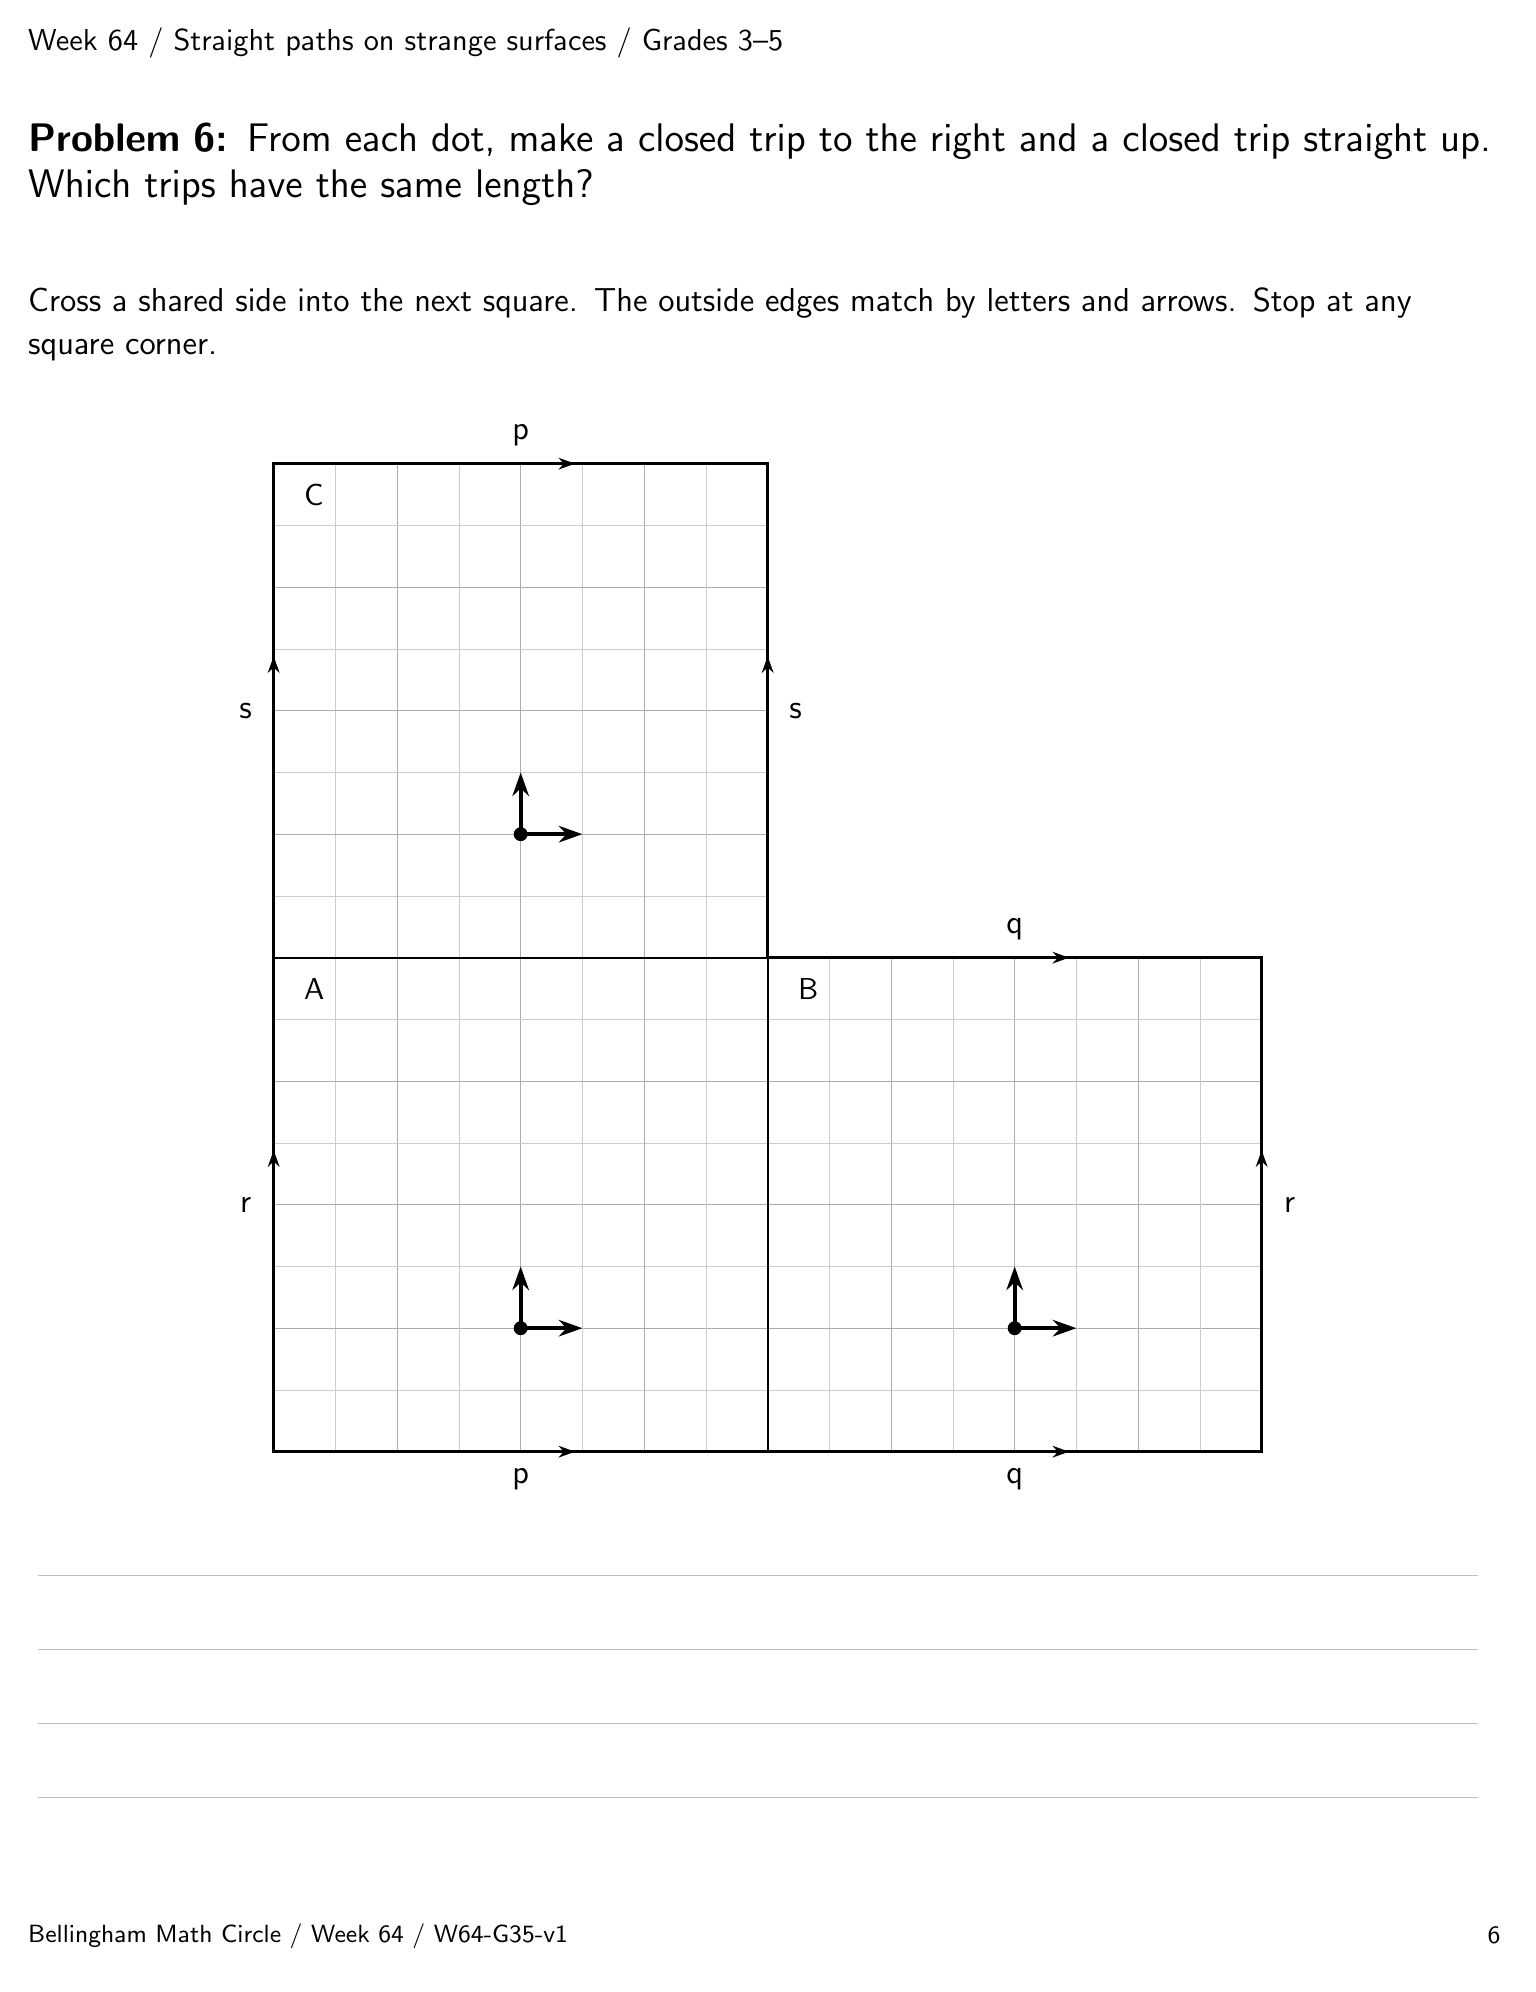
\begin{tikzpicture}[x=1in,y=-1in]
\path[use as bounding box] (0,0) rectangle (7.4,9.68);
\node[anchor=north west,inner sep=0pt,align=left,text width=7.4in,font=\fontsize{10.6}{13.25}\selectfont] at (0.00000,0.00000) {Week 64 / Straight paths on strange surfaces / Grades 3--5};
\node[anchor=north west,inner sep=0pt,align=left,text width=6.8in,font=\fontsize{9.5}{11.88}\selectfont] at (0.00000,9.48000) {Bellingham Math Circle / Week 64 / W64-G35-v1};
\node[anchor=east,inner sep=1pt,font=\fontsize{9.5}{10.5}\selectfont] at (7.38000,9.54000) {6};
\node[anchor=north west,inner sep=0pt,align=left,text width=7.35in,font=\fontsize{13.3}{16.62}\selectfont] at (0.00000,0.48000) {\textbf{Problem 6:} From each dot, make a closed trip to the right and a closed trip straight up. Which trips have the same length?};
\node[anchor=north west,inner sep=0pt,align=left,text width=7.35in,font=\fontsize{12.5}{15.62}\selectfont] at (0.00000,1.30000) {Cross a shared side into the next square. The outside edges match by letters and arrows. Stop at any square corner.};
\draw[black!20,line width=.25pt] (1.53875,7.12000) -- (1.53875,4.65000);
\draw[black!20,line width=.25pt] (1.23000,6.81125) -- (3.70000,6.81125);
\draw[black!32,line width=.35pt] (1.84750,7.12000) -- (1.84750,4.65000);
\draw[black!32,line width=.35pt] (1.23000,6.50250) -- (3.70000,6.50250);
\draw[black!20,line width=.25pt] (2.15625,7.12000) -- (2.15625,4.65000);
\draw[black!20,line width=.25pt] (1.23000,6.19375) -- (3.70000,6.19375);
\draw[black!32,line width=.35pt] (2.46500,7.12000) -- (2.46500,4.65000);
\draw[black!32,line width=.35pt] (1.23000,5.88500) -- (3.70000,5.88500);
\draw[black!20,line width=.25pt] (2.77375,7.12000) -- (2.77375,4.65000);
\draw[black!20,line width=.25pt] (1.23000,5.57625) -- (3.70000,5.57625);
\draw[black!32,line width=.35pt] (3.08250,7.12000) -- (3.08250,4.65000);
\draw[black!32,line width=.35pt] (1.23000,5.26750) -- (3.70000,5.26750);
\draw[black!20,line width=.25pt] (3.39125,7.12000) -- (3.39125,4.65000);
\draw[black!20,line width=.25pt] (1.23000,4.95875) -- (3.70000,4.95875);
\node[anchor=north west,inner sep=1pt,font=\fontsize{11}{12}\selectfont] at (1.36585,4.73645) {A};
\draw[black!20,line width=.25pt] (4.00875,7.12000) -- (4.00875,4.65000);
\draw[black!20,line width=.25pt] (3.70000,6.81125) -- (6.17000,6.81125);
\draw[black!32,line width=.35pt] (4.31750,7.12000) -- (4.31750,4.65000);
\draw[black!32,line width=.35pt] (3.70000,6.50250) -- (6.17000,6.50250);
\draw[black!20,line width=.25pt] (4.62625,7.12000) -- (4.62625,4.65000);
\draw[black!20,line width=.25pt] (3.70000,6.19375) -- (6.17000,6.19375);
\draw[black!32,line width=.35pt] (4.93500,7.12000) -- (4.93500,4.65000);
\draw[black!32,line width=.35pt] (3.70000,5.88500) -- (6.17000,5.88500);
\draw[black!20,line width=.25pt] (5.24375,7.12000) -- (5.24375,4.65000);
\draw[black!20,line width=.25pt] (3.70000,5.57625) -- (6.17000,5.57625);
\draw[black!32,line width=.35pt] (5.55250,7.12000) -- (5.55250,4.65000);
\draw[black!32,line width=.35pt] (3.70000,5.26750) -- (6.17000,5.26750);
\draw[black!20,line width=.25pt] (5.86125,7.12000) -- (5.86125,4.65000);
\draw[black!20,line width=.25pt] (3.70000,4.95875) -- (6.17000,4.95875);
\node[anchor=north west,inner sep=1pt,font=\fontsize{11}{12}\selectfont] at (3.83585,4.73645) {B};
\draw[black!20,line width=.25pt] (1.53875,4.65000) -- (1.53875,2.18000);
\draw[black!20,line width=.25pt] (1.23000,4.34125) -- (3.70000,4.34125);
\draw[black!32,line width=.35pt] (1.84750,4.65000) -- (1.84750,2.18000);
\draw[black!32,line width=.35pt] (1.23000,4.03250) -- (3.70000,4.03250);
\draw[black!20,line width=.25pt] (2.15625,4.65000) -- (2.15625,2.18000);
\draw[black!20,line width=.25pt] (1.23000,3.72375) -- (3.70000,3.72375);
\draw[black!32,line width=.35pt] (2.46500,4.65000) -- (2.46500,2.18000);
\draw[black!32,line width=.35pt] (1.23000,3.41500) -- (3.70000,3.41500);
\draw[black!20,line width=.25pt] (2.77375,4.65000) -- (2.77375,2.18000);
\draw[black!20,line width=.25pt] (1.23000,3.10625) -- (3.70000,3.10625);
\draw[black!32,line width=.35pt] (3.08250,4.65000) -- (3.08250,2.18000);
\draw[black!32,line width=.35pt] (1.23000,2.79750) -- (3.70000,2.79750);
\draw[black!20,line width=.25pt] (3.39125,4.65000) -- (3.39125,2.18000);
\draw[black!20,line width=.25pt] (1.23000,2.48875) -- (3.70000,2.48875);
\node[anchor=north west,inner sep=1pt,font=\fontsize{11}{12}\selectfont] at (1.36585,2.26645) {C};
\draw[line width=.95pt] (1.23000,7.12000) -- (6.17000,7.12000) -- (6.17000,4.65000) -- (3.70000,4.65000) -- (3.70000,2.18000) -- (1.23000,2.18000) -- cycle;
\draw[line width=.8pt] (3.70000,7.12000) -- (3.70000,4.65000);
\draw[line width=.8pt] (1.23000,4.65000) -- (3.70000,4.65000);
\draw[edge] (2.19330,7.12000) -- (2.73670,7.12000);
\node[anchor=center,inner sep=1pt,font=\fontsize{12}{13}\selectfont] at (2.46500,7.26000) {p};
\draw[edge] (2.19330,2.18000) -- (2.73670,2.18000);
\node[anchor=center,inner sep=1pt,font=\fontsize{12}{13}\selectfont] at (2.46500,2.04000) {p};
\draw[edge] (4.66330,7.12000) -- (5.20670,7.12000);
\node[anchor=center,inner sep=1pt,font=\fontsize{12}{13}\selectfont] at (4.93500,7.26000) {q};
\draw[edge] (4.66330,4.65000) -- (5.20670,4.65000);
\node[anchor=center,inner sep=1pt,font=\fontsize{12}{13}\selectfont] at (4.93500,4.51000) {q};
\draw[edge] (1.23000,6.15670) -- (1.23000,5.61330);
\node[anchor=center,inner sep=1pt,font=\fontsize{12}{13}\selectfont] at (1.09000,5.88500) {r};
\draw[edge] (6.17000,6.15670) -- (6.17000,5.61330);
\node[anchor=center,inner sep=1pt,font=\fontsize{12}{13}\selectfont] at (6.31000,5.88500) {r};
\draw[edge] (1.23000,3.68670) -- (1.23000,3.14330);
\node[anchor=center,inner sep=1pt,font=\fontsize{12}{13}\selectfont] at (1.09000,3.41500) {s};
\draw[edge] (3.70000,3.68670) -- (3.70000,3.14330);
\node[anchor=center,inner sep=1pt,font=\fontsize{12}{13}\selectfont] at (3.84000,3.41500) {s};
\draw[fill=black] (2.46500,6.50250) circle[radius=.032in];
\draw[travel] (2.46500,6.50250) -- (2.77375,6.50250);
\draw[travel] (2.46500,6.50250) -- (2.46500,6.19375);
\draw[fill=black] (4.93500,6.50250) circle[radius=.032in];
\draw[travel] (4.93500,6.50250) -- (5.24375,6.50250);
\draw[travel] (4.93500,6.50250) -- (4.93500,6.19375);
\draw[fill=black] (2.46500,4.03250) circle[radius=.032in];
\draw[travel] (2.46500,4.03250) -- (2.77375,4.03250);
\draw[travel] (2.46500,4.03250) -- (2.46500,3.72375);
\draw[black!25,line width=.35pt] (0.05000,7.74000) -- (7.25000,7.74000);
\draw[black!25,line width=.35pt] (0.05000,8.11000) -- (7.25000,8.11000);
\draw[black!25,line width=.35pt] (0.05000,8.48000) -- (7.25000,8.48000);
\draw[black!25,line width=.35pt] (0.05000,8.85000) -- (7.25000,8.85000);
\end{tikzpicture}\newpage
\noindent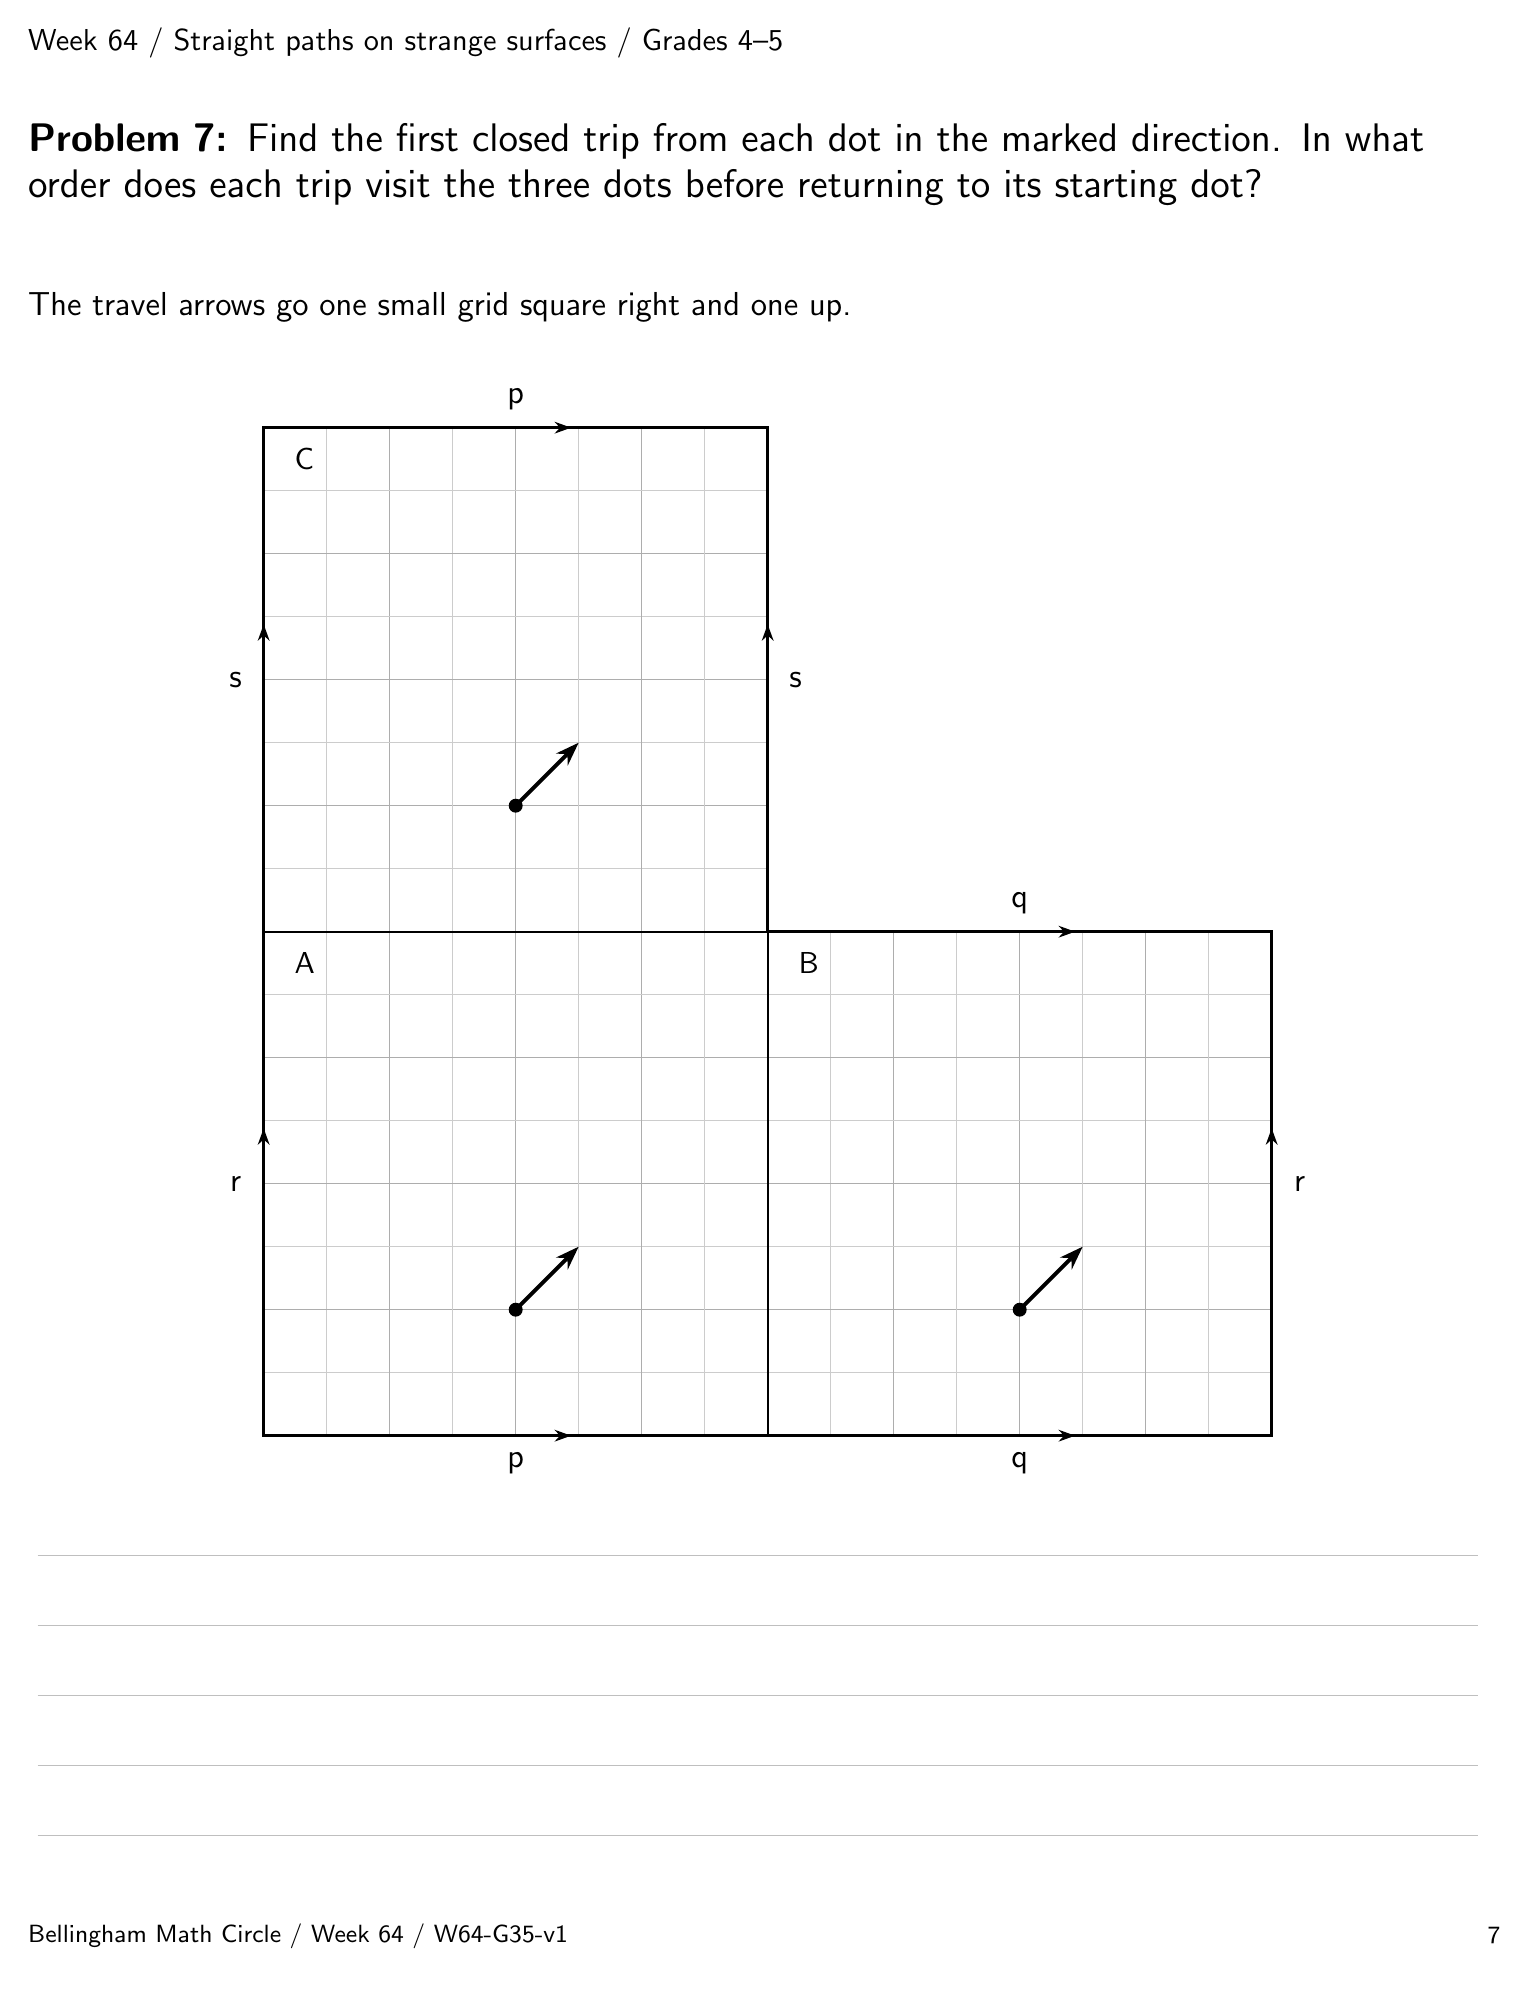
\begin{tikzpicture}[x=1in,y=-1in]
\path[use as bounding box] (0,0) rectangle (7.4,9.68);
\node[anchor=north west,inner sep=0pt,align=left,text width=7.4in,font=\fontsize{10.6}{13.25}\selectfont] at (0.00000,0.00000) {Week 64 / Straight paths on strange surfaces / Grades 4--5};
\node[anchor=north west,inner sep=0pt,align=left,text width=6.8in,font=\fontsize{9.5}{11.88}\selectfont] at (0.00000,9.48000) {Bellingham Math Circle / Week 64 / W64-G35-v1};
\node[anchor=east,inner sep=1pt,font=\fontsize{9.5}{10.5}\selectfont] at (7.38000,9.54000) {7};
\node[anchor=north west,inner sep=0pt,align=left,text width=7.35in,font=\fontsize{13.3}{16.62}\selectfont] at (0.00000,0.48000) {\textbf{Problem 7:} Find the first closed trip from each dot in the marked direction. In what order does each trip visit the three dots before returning to its starting dot?};
\node[anchor=north west,inner sep=0pt,align=left,text width=7.3in,font=\fontsize{12.5}{15.62}\selectfont] at (0.00000,1.32000) {The travel arrows go one small grid square right and one up.};
\draw[black!20,line width=.25pt] (1.49500,7.04000) -- (1.49500,4.52000);
\draw[black!20,line width=.25pt] (1.18000,6.72500) -- (3.70000,6.72500);
\draw[black!32,line width=.35pt] (1.81000,7.04000) -- (1.81000,4.52000);
\draw[black!32,line width=.35pt] (1.18000,6.41000) -- (3.70000,6.41000);
\draw[black!20,line width=.25pt] (2.12500,7.04000) -- (2.12500,4.52000);
\draw[black!20,line width=.25pt] (1.18000,6.09500) -- (3.70000,6.09500);
\draw[black!32,line width=.35pt] (2.44000,7.04000) -- (2.44000,4.52000);
\draw[black!32,line width=.35pt] (1.18000,5.78000) -- (3.70000,5.78000);
\draw[black!20,line width=.25pt] (2.75500,7.04000) -- (2.75500,4.52000);
\draw[black!20,line width=.25pt] (1.18000,5.46500) -- (3.70000,5.46500);
\draw[black!32,line width=.35pt] (3.07000,7.04000) -- (3.07000,4.52000);
\draw[black!32,line width=.35pt] (1.18000,5.15000) -- (3.70000,5.15000);
\draw[black!20,line width=.25pt] (3.38500,7.04000) -- (3.38500,4.52000);
\draw[black!20,line width=.25pt] (1.18000,4.83500) -- (3.70000,4.83500);
\node[anchor=north west,inner sep=1pt,font=\fontsize{11}{12}\selectfont] at (1.31860,4.60820) {A};
\draw[black!20,line width=.25pt] (4.01500,7.04000) -- (4.01500,4.52000);
\draw[black!20,line width=.25pt] (3.70000,6.72500) -- (6.22000,6.72500);
\draw[black!32,line width=.35pt] (4.33000,7.04000) -- (4.33000,4.52000);
\draw[black!32,line width=.35pt] (3.70000,6.41000) -- (6.22000,6.41000);
\draw[black!20,line width=.25pt] (4.64500,7.04000) -- (4.64500,4.52000);
\draw[black!20,line width=.25pt] (3.70000,6.09500) -- (6.22000,6.09500);
\draw[black!32,line width=.35pt] (4.96000,7.04000) -- (4.96000,4.52000);
\draw[black!32,line width=.35pt] (3.70000,5.78000) -- (6.22000,5.78000);
\draw[black!20,line width=.25pt] (5.27500,7.04000) -- (5.27500,4.52000);
\draw[black!20,line width=.25pt] (3.70000,5.46500) -- (6.22000,5.46500);
\draw[black!32,line width=.35pt] (5.59000,7.04000) -- (5.59000,4.52000);
\draw[black!32,line width=.35pt] (3.70000,5.15000) -- (6.22000,5.15000);
\draw[black!20,line width=.25pt] (5.90500,7.04000) -- (5.90500,4.52000);
\draw[black!20,line width=.25pt] (3.70000,4.83500) -- (6.22000,4.83500);
\node[anchor=north west,inner sep=1pt,font=\fontsize{11}{12}\selectfont] at (3.83860,4.60820) {B};
\draw[black!20,line width=.25pt] (1.49500,4.52000) -- (1.49500,2.00000);
\draw[black!20,line width=.25pt] (1.18000,4.20500) -- (3.70000,4.20500);
\draw[black!32,line width=.35pt] (1.81000,4.52000) -- (1.81000,2.00000);
\draw[black!32,line width=.35pt] (1.18000,3.89000) -- (3.70000,3.89000);
\draw[black!20,line width=.25pt] (2.12500,4.52000) -- (2.12500,2.00000);
\draw[black!20,line width=.25pt] (1.18000,3.57500) -- (3.70000,3.57500);
\draw[black!32,line width=.35pt] (2.44000,4.52000) -- (2.44000,2.00000);
\draw[black!32,line width=.35pt] (1.18000,3.26000) -- (3.70000,3.26000);
\draw[black!20,line width=.25pt] (2.75500,4.52000) -- (2.75500,2.00000);
\draw[black!20,line width=.25pt] (1.18000,2.94500) -- (3.70000,2.94500);
\draw[black!32,line width=.35pt] (3.07000,4.52000) -- (3.07000,2.00000);
\draw[black!32,line width=.35pt] (1.18000,2.63000) -- (3.70000,2.63000);
\draw[black!20,line width=.25pt] (3.38500,4.52000) -- (3.38500,2.00000);
\draw[black!20,line width=.25pt] (1.18000,2.31500) -- (3.70000,2.31500);
\node[anchor=north west,inner sep=1pt,font=\fontsize{11}{12}\selectfont] at (1.31860,2.08820) {C};
\draw[line width=.95pt] (1.18000,7.04000) -- (6.22000,7.04000) -- (6.22000,4.52000) -- (3.70000,4.52000) -- (3.70000,2.00000) -- (1.18000,2.00000) -- cycle;
\draw[line width=.8pt] (3.70000,7.04000) -- (3.70000,4.52000);
\draw[line width=.8pt] (1.18000,4.52000) -- (3.70000,4.52000);
\draw[edge] (2.16280,7.04000) -- (2.71720,7.04000);
\node[anchor=center,inner sep=1pt,font=\fontsize{12}{13}\selectfont] at (2.44000,7.18000) {p};
\draw[edge] (2.16280,2.00000) -- (2.71720,2.00000);
\node[anchor=center,inner sep=1pt,font=\fontsize{12}{13}\selectfont] at (2.44000,1.86000) {p};
\draw[edge] (4.68280,7.04000) -- (5.23720,7.04000);
\node[anchor=center,inner sep=1pt,font=\fontsize{12}{13}\selectfont] at (4.96000,7.18000) {q};
\draw[edge] (4.68280,4.52000) -- (5.23720,4.52000);
\node[anchor=center,inner sep=1pt,font=\fontsize{12}{13}\selectfont] at (4.96000,4.38000) {q};
\draw[edge] (1.18000,6.05720) -- (1.18000,5.50280);
\node[anchor=center,inner sep=1pt,font=\fontsize{12}{13}\selectfont] at (1.04000,5.78000) {r};
\draw[edge] (6.22000,6.05720) -- (6.22000,5.50280);
\node[anchor=center,inner sep=1pt,font=\fontsize{12}{13}\selectfont] at (6.36000,5.78000) {r};
\draw[edge] (1.18000,3.53720) -- (1.18000,2.98280);
\node[anchor=center,inner sep=1pt,font=\fontsize{12}{13}\selectfont] at (1.04000,3.26000) {s};
\draw[edge] (3.70000,3.53720) -- (3.70000,2.98280);
\node[anchor=center,inner sep=1pt,font=\fontsize{12}{13}\selectfont] at (3.84000,3.26000) {s};
\draw[fill=black] (2.44000,6.41000) circle[radius=.032in];
\draw[travel] (2.44000,6.41000) -- (2.75500,6.09500);
\draw[fill=black] (4.96000,6.41000) circle[radius=.032in];
\draw[travel] (4.96000,6.41000) -- (5.27500,6.09500);
\draw[fill=black] (2.44000,3.89000) circle[radius=.032in];
\draw[travel] (2.44000,3.89000) -- (2.75500,3.57500);
\draw[black!25,line width=.35pt] (0.05000,7.64000) -- (7.25000,7.64000);
\draw[black!25,line width=.35pt] (0.05000,7.99000) -- (7.25000,7.99000);
\draw[black!25,line width=.35pt] (0.05000,8.34000) -- (7.25000,8.34000);
\draw[black!25,line width=.35pt] (0.05000,8.69000) -- (7.25000,8.69000);
\draw[black!25,line width=.35pt] (0.05000,9.04000) -- (7.25000,9.04000);
\end{tikzpicture}\newpage
\noindent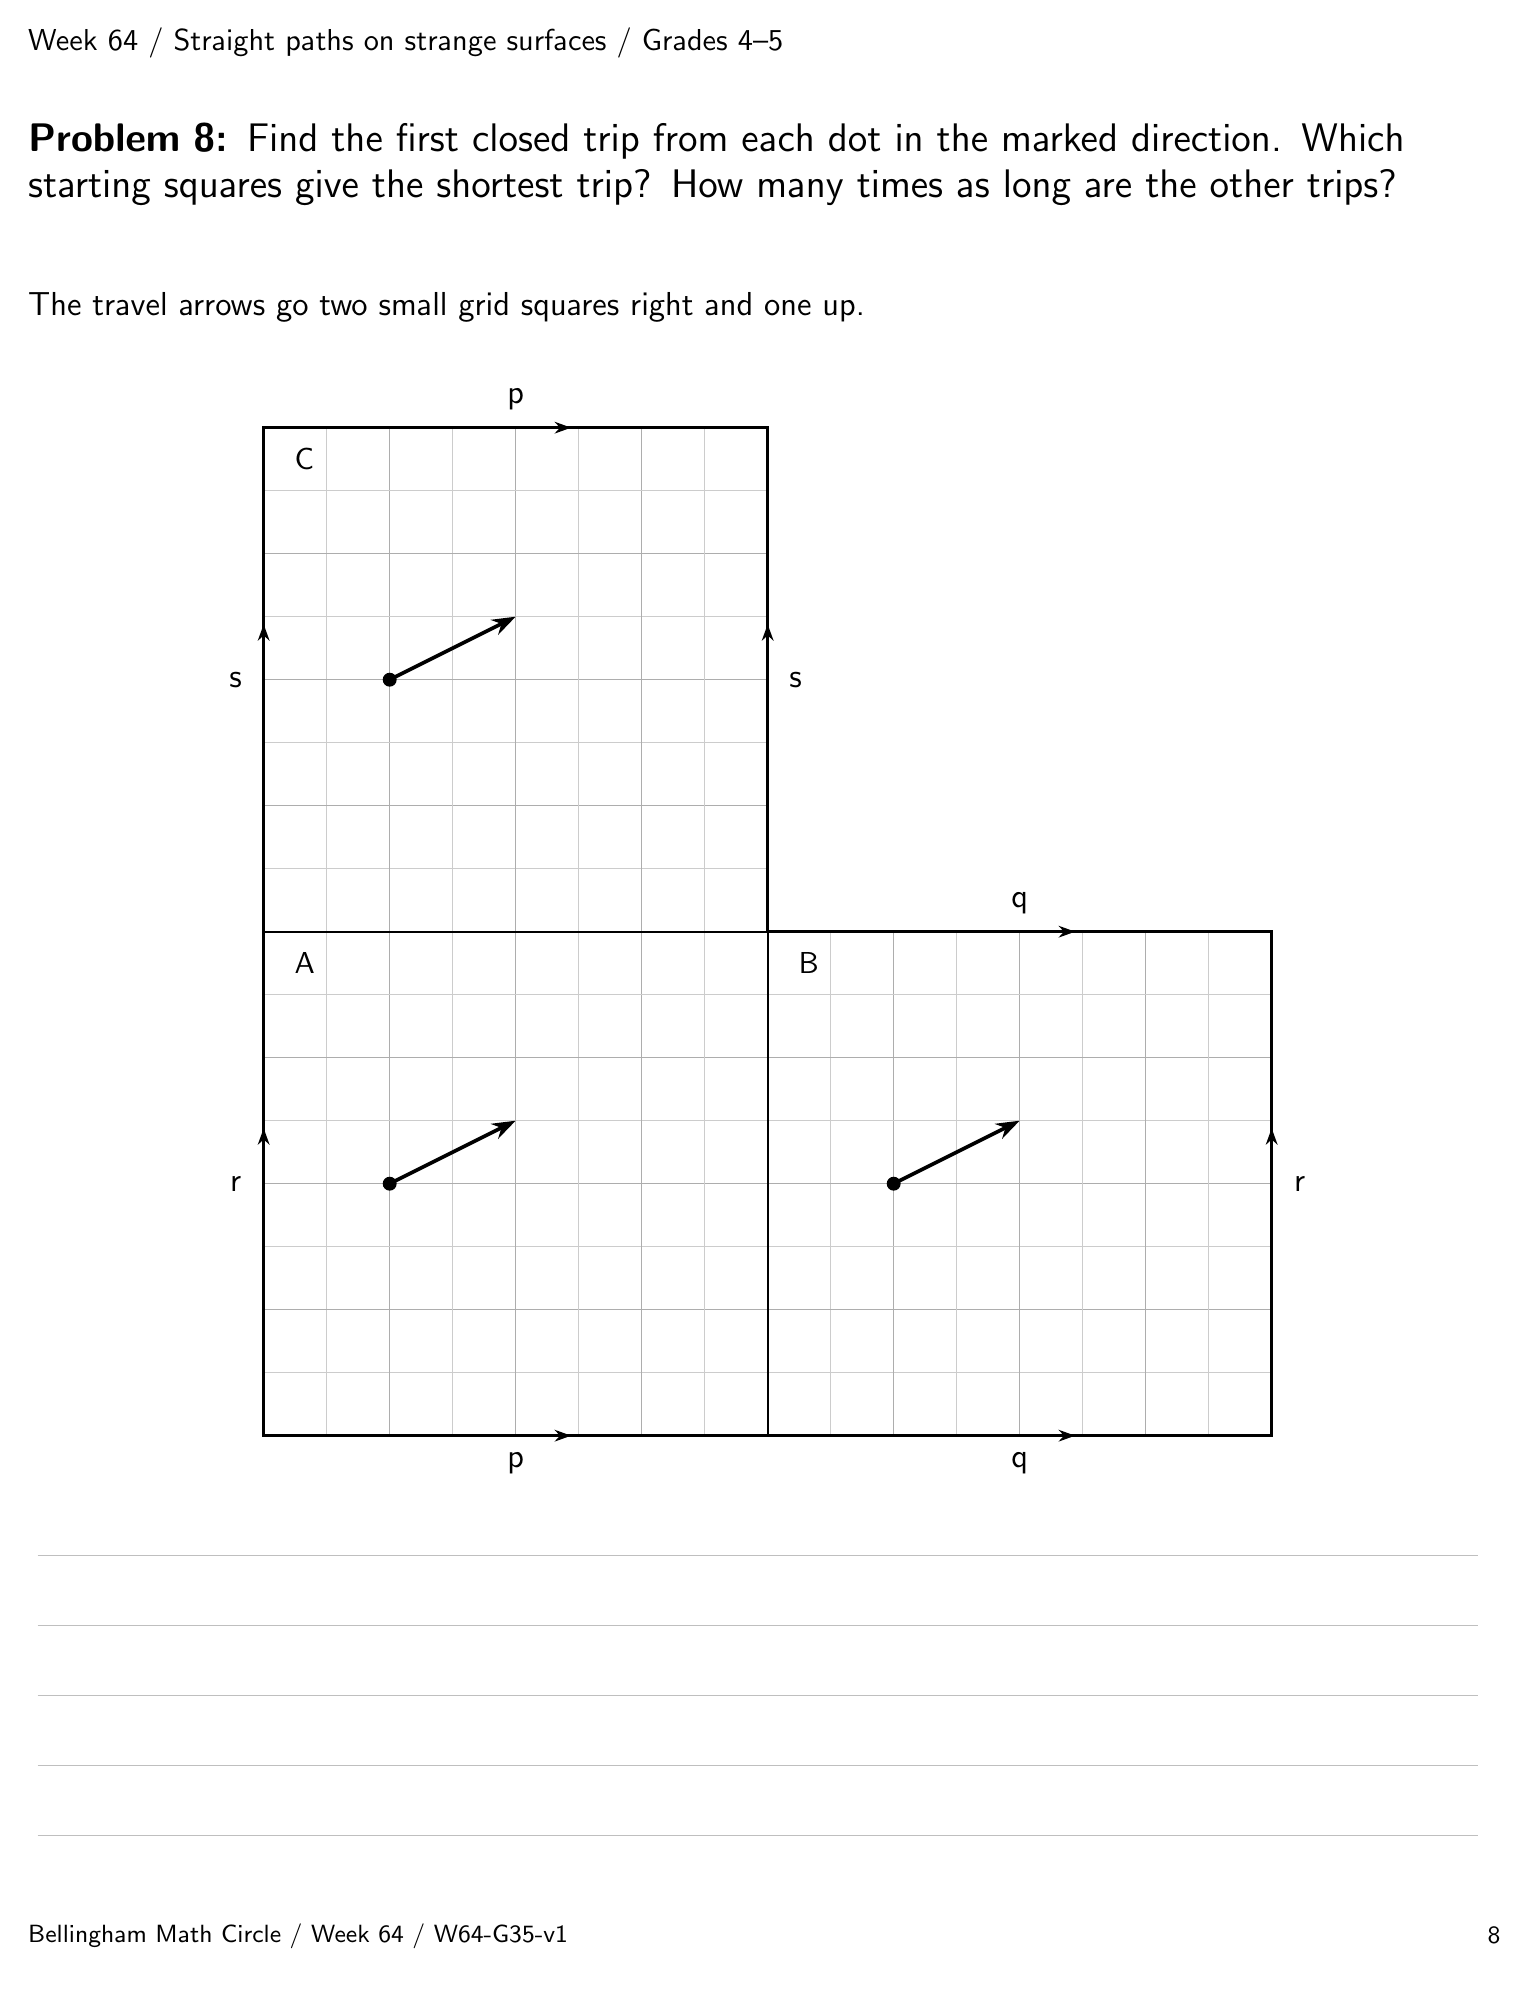
\begin{tikzpicture}[x=1in,y=-1in]
\path[use as bounding box] (0,0) rectangle (7.4,9.68);
\node[anchor=north west,inner sep=0pt,align=left,text width=7.4in,font=\fontsize{10.6}{13.25}\selectfont] at (0.00000,0.00000) {Week 64 / Straight paths on strange surfaces / Grades 4--5};
\node[anchor=north west,inner sep=0pt,align=left,text width=6.8in,font=\fontsize{9.5}{11.88}\selectfont] at (0.00000,9.48000) {Bellingham Math Circle / Week 64 / W64-G35-v1};
\node[anchor=east,inner sep=1pt,font=\fontsize{9.5}{10.5}\selectfont] at (7.38000,9.54000) {8};
\node[anchor=north west,inner sep=0pt,align=left,text width=7.35in,font=\fontsize{13.3}{16.62}\selectfont] at (0.00000,0.48000) {\textbf{Problem 8:} Find the first closed trip from each dot in the marked direction. Which starting squares give the shortest trip? How many times as long are the other trips?};
\node[anchor=north west,inner sep=0pt,align=left,text width=7.3in,font=\fontsize{12.5}{15.62}\selectfont] at (0.00000,1.32000) {The travel arrows go two small grid squares right and one up.};
\draw[black!20,line width=.25pt] (1.49500,7.04000) -- (1.49500,4.52000);
\draw[black!20,line width=.25pt] (1.18000,6.72500) -- (3.70000,6.72500);
\draw[black!32,line width=.35pt] (1.81000,7.04000) -- (1.81000,4.52000);
\draw[black!32,line width=.35pt] (1.18000,6.41000) -- (3.70000,6.41000);
\draw[black!20,line width=.25pt] (2.12500,7.04000) -- (2.12500,4.52000);
\draw[black!20,line width=.25pt] (1.18000,6.09500) -- (3.70000,6.09500);
\draw[black!32,line width=.35pt] (2.44000,7.04000) -- (2.44000,4.52000);
\draw[black!32,line width=.35pt] (1.18000,5.78000) -- (3.70000,5.78000);
\draw[black!20,line width=.25pt] (2.75500,7.04000) -- (2.75500,4.52000);
\draw[black!20,line width=.25pt] (1.18000,5.46500) -- (3.70000,5.46500);
\draw[black!32,line width=.35pt] (3.07000,7.04000) -- (3.07000,4.52000);
\draw[black!32,line width=.35pt] (1.18000,5.15000) -- (3.70000,5.15000);
\draw[black!20,line width=.25pt] (3.38500,7.04000) -- (3.38500,4.52000);
\draw[black!20,line width=.25pt] (1.18000,4.83500) -- (3.70000,4.83500);
\node[anchor=north west,inner sep=1pt,font=\fontsize{11}{12}\selectfont] at (1.31860,4.60820) {A};
\draw[black!20,line width=.25pt] (4.01500,7.04000) -- (4.01500,4.52000);
\draw[black!20,line width=.25pt] (3.70000,6.72500) -- (6.22000,6.72500);
\draw[black!32,line width=.35pt] (4.33000,7.04000) -- (4.33000,4.52000);
\draw[black!32,line width=.35pt] (3.70000,6.41000) -- (6.22000,6.41000);
\draw[black!20,line width=.25pt] (4.64500,7.04000) -- (4.64500,4.52000);
\draw[black!20,line width=.25pt] (3.70000,6.09500) -- (6.22000,6.09500);
\draw[black!32,line width=.35pt] (4.96000,7.04000) -- (4.96000,4.52000);
\draw[black!32,line width=.35pt] (3.70000,5.78000) -- (6.22000,5.78000);
\draw[black!20,line width=.25pt] (5.27500,7.04000) -- (5.27500,4.52000);
\draw[black!20,line width=.25pt] (3.70000,5.46500) -- (6.22000,5.46500);
\draw[black!32,line width=.35pt] (5.59000,7.04000) -- (5.59000,4.52000);
\draw[black!32,line width=.35pt] (3.70000,5.15000) -- (6.22000,5.15000);
\draw[black!20,line width=.25pt] (5.90500,7.04000) -- (5.90500,4.52000);
\draw[black!20,line width=.25pt] (3.70000,4.83500) -- (6.22000,4.83500);
\node[anchor=north west,inner sep=1pt,font=\fontsize{11}{12}\selectfont] at (3.83860,4.60820) {B};
\draw[black!20,line width=.25pt] (1.49500,4.52000) -- (1.49500,2.00000);
\draw[black!20,line width=.25pt] (1.18000,4.20500) -- (3.70000,4.20500);
\draw[black!32,line width=.35pt] (1.81000,4.52000) -- (1.81000,2.00000);
\draw[black!32,line width=.35pt] (1.18000,3.89000) -- (3.70000,3.89000);
\draw[black!20,line width=.25pt] (2.12500,4.52000) -- (2.12500,2.00000);
\draw[black!20,line width=.25pt] (1.18000,3.57500) -- (3.70000,3.57500);
\draw[black!32,line width=.35pt] (2.44000,4.52000) -- (2.44000,2.00000);
\draw[black!32,line width=.35pt] (1.18000,3.26000) -- (3.70000,3.26000);
\draw[black!20,line width=.25pt] (2.75500,4.52000) -- (2.75500,2.00000);
\draw[black!20,line width=.25pt] (1.18000,2.94500) -- (3.70000,2.94500);
\draw[black!32,line width=.35pt] (3.07000,4.52000) -- (3.07000,2.00000);
\draw[black!32,line width=.35pt] (1.18000,2.63000) -- (3.70000,2.63000);
\draw[black!20,line width=.25pt] (3.38500,4.52000) -- (3.38500,2.00000);
\draw[black!20,line width=.25pt] (1.18000,2.31500) -- (3.70000,2.31500);
\node[anchor=north west,inner sep=1pt,font=\fontsize{11}{12}\selectfont] at (1.31860,2.08820) {C};
\draw[line width=.95pt] (1.18000,7.04000) -- (6.22000,7.04000) -- (6.22000,4.52000) -- (3.70000,4.52000) -- (3.70000,2.00000) -- (1.18000,2.00000) -- cycle;
\draw[line width=.8pt] (3.70000,7.04000) -- (3.70000,4.52000);
\draw[line width=.8pt] (1.18000,4.52000) -- (3.70000,4.52000);
\draw[edge] (2.16280,7.04000) -- (2.71720,7.04000);
\node[anchor=center,inner sep=1pt,font=\fontsize{12}{13}\selectfont] at (2.44000,7.18000) {p};
\draw[edge] (2.16280,2.00000) -- (2.71720,2.00000);
\node[anchor=center,inner sep=1pt,font=\fontsize{12}{13}\selectfont] at (2.44000,1.86000) {p};
\draw[edge] (4.68280,7.04000) -- (5.23720,7.04000);
\node[anchor=center,inner sep=1pt,font=\fontsize{12}{13}\selectfont] at (4.96000,7.18000) {q};
\draw[edge] (4.68280,4.52000) -- (5.23720,4.52000);
\node[anchor=center,inner sep=1pt,font=\fontsize{12}{13}\selectfont] at (4.96000,4.38000) {q};
\draw[edge] (1.18000,6.05720) -- (1.18000,5.50280);
\node[anchor=center,inner sep=1pt,font=\fontsize{12}{13}\selectfont] at (1.04000,5.78000) {r};
\draw[edge] (6.22000,6.05720) -- (6.22000,5.50280);
\node[anchor=center,inner sep=1pt,font=\fontsize{12}{13}\selectfont] at (6.36000,5.78000) {r};
\draw[edge] (1.18000,3.53720) -- (1.18000,2.98280);
\node[anchor=center,inner sep=1pt,font=\fontsize{12}{13}\selectfont] at (1.04000,3.26000) {s};
\draw[edge] (3.70000,3.53720) -- (3.70000,2.98280);
\node[anchor=center,inner sep=1pt,font=\fontsize{12}{13}\selectfont] at (3.84000,3.26000) {s};
\draw[fill=black] (1.81000,5.78000) circle[radius=.032in];
\draw[travel] (1.81000,5.78000) -- (2.44000,5.46500);
\draw[fill=black] (4.33000,5.78000) circle[radius=.032in];
\draw[travel] (4.33000,5.78000) -- (4.96000,5.46500);
\draw[fill=black] (1.81000,3.26000) circle[radius=.032in];
\draw[travel] (1.81000,3.26000) -- (2.44000,2.94500);
\draw[black!25,line width=.35pt] (0.05000,7.64000) -- (7.25000,7.64000);
\draw[black!25,line width=.35pt] (0.05000,7.99000) -- (7.25000,7.99000);
\draw[black!25,line width=.35pt] (0.05000,8.34000) -- (7.25000,8.34000);
\draw[black!25,line width=.35pt] (0.05000,8.69000) -- (7.25000,8.69000);
\draw[black!25,line width=.35pt] (0.05000,9.04000) -- (7.25000,9.04000);
\end{tikzpicture}\newpage
\noindent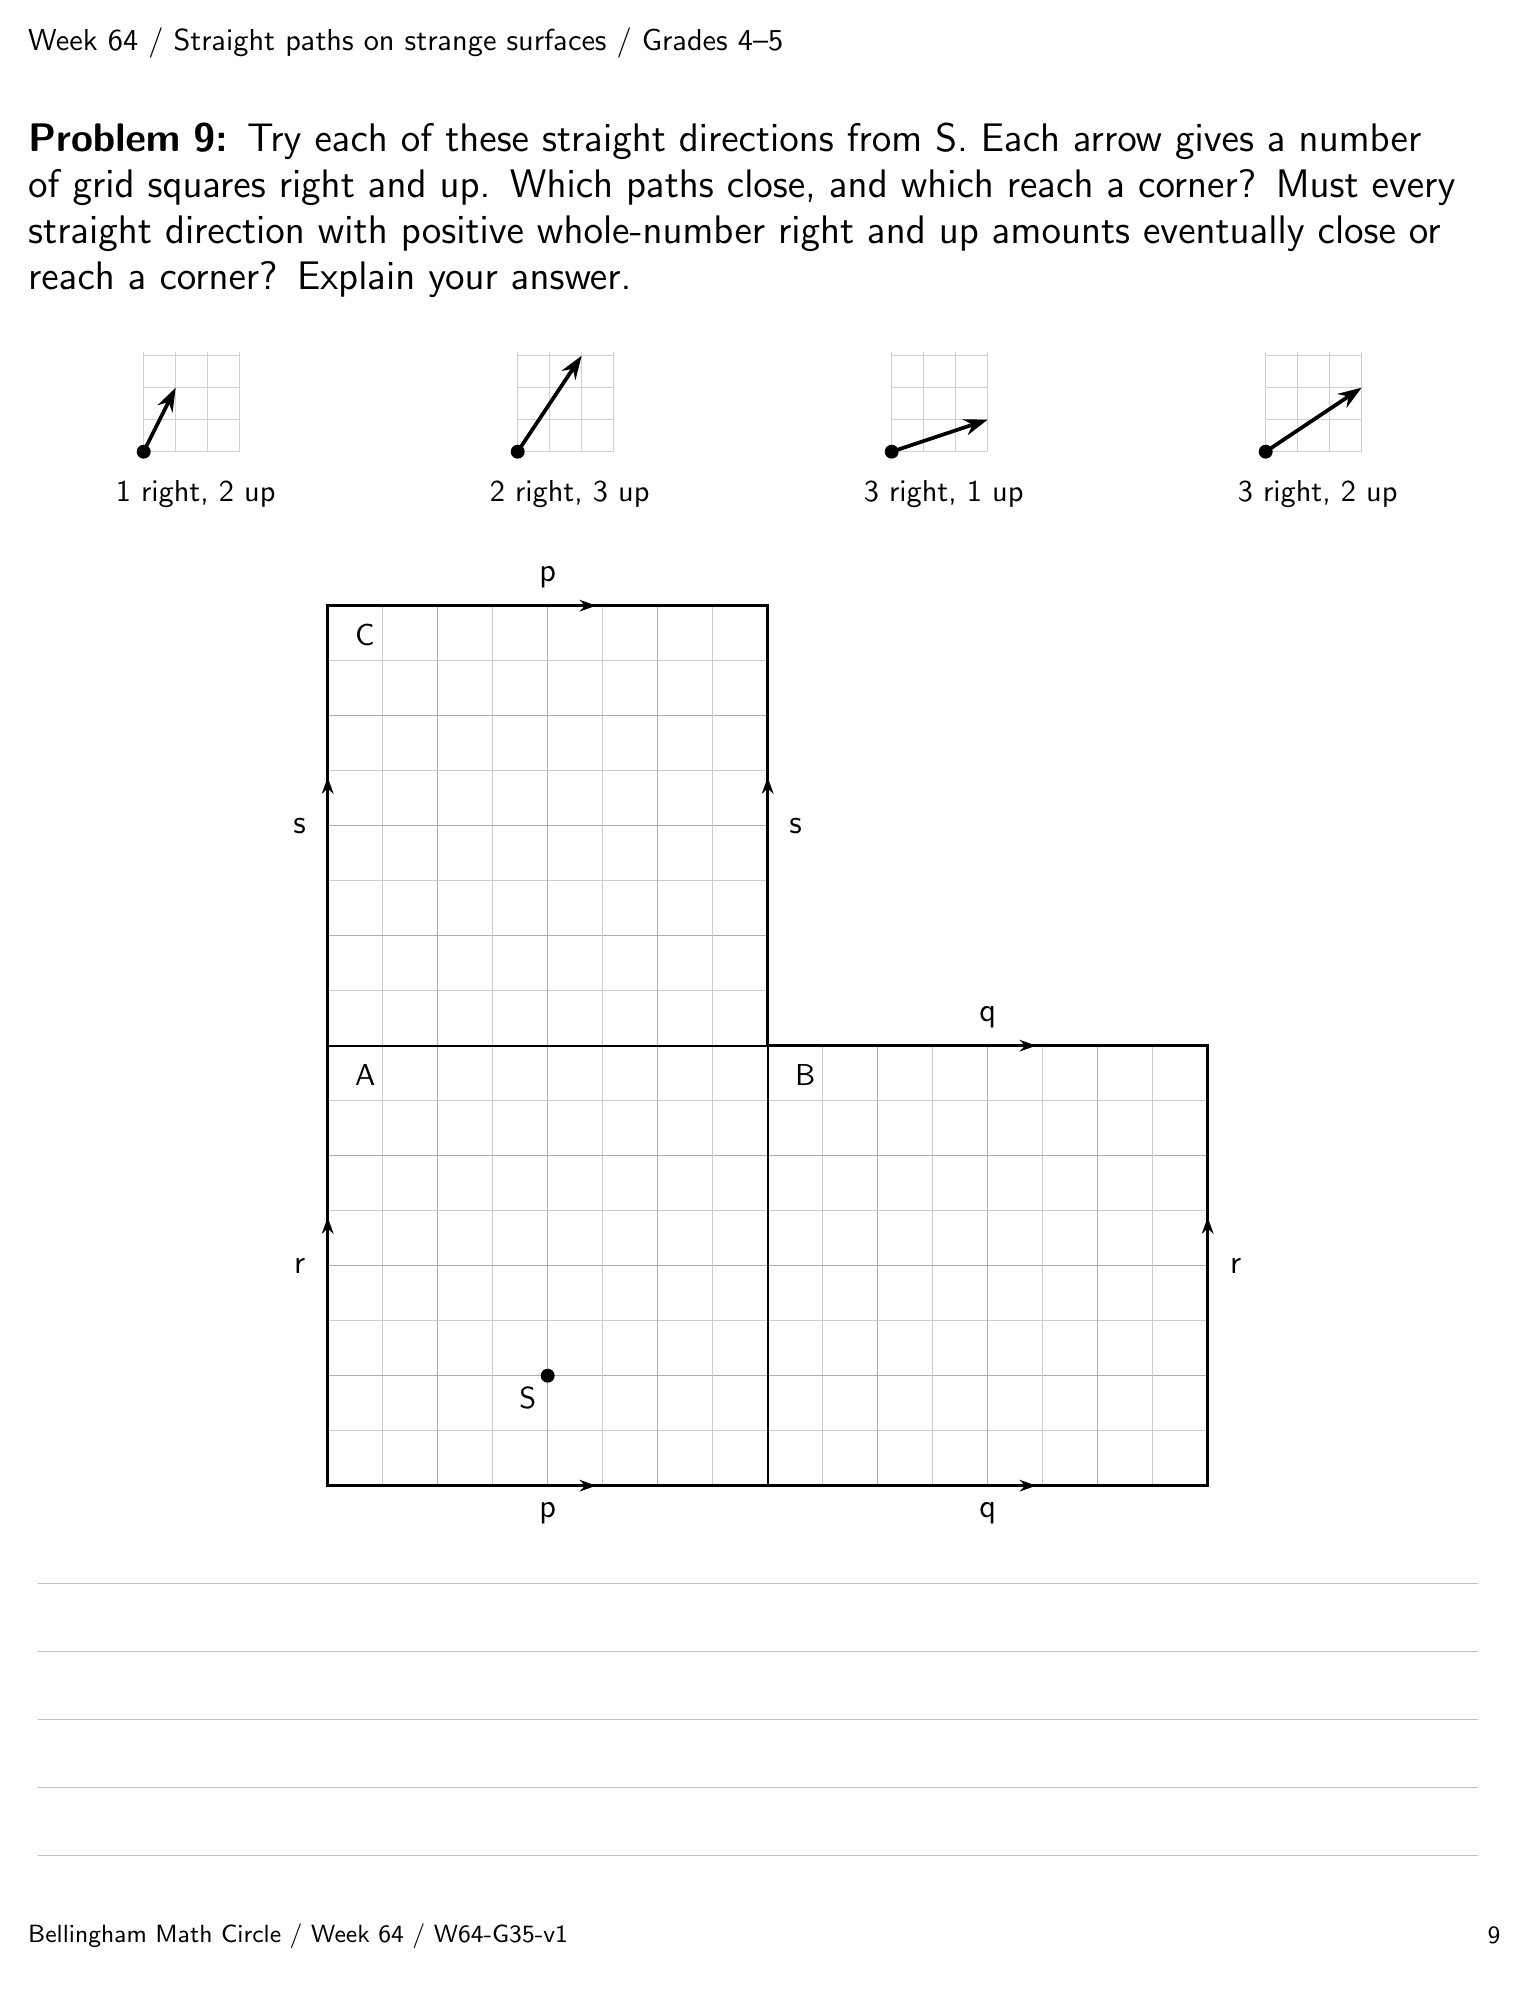
\begin{tikzpicture}[x=1in,y=-1in]
\path[use as bounding box] (0,0) rectangle (7.4,9.68);
\node[anchor=north west,inner sep=0pt,align=left,text width=7.4in,font=\fontsize{10.6}{13.25}\selectfont] at (0.00000,0.00000) {Week 64 / Straight paths on strange surfaces / Grades 4--5};
\node[anchor=north west,inner sep=0pt,align=left,text width=6.8in,font=\fontsize{9.5}{11.88}\selectfont] at (0.00000,9.48000) {Bellingham Math Circle / Week 64 / W64-G35-v1};
\node[anchor=east,inner sep=1pt,font=\fontsize{9.5}{10.5}\selectfont] at (7.38000,9.54000) {9};
\node[anchor=north west,inner sep=0pt,align=left,text width=7.35in,font=\fontsize{13.3}{16.62}\selectfont] at (0.00000,0.48000) {\textbf{Problem 9:} Try each of these straight directions from S. Each arrow gives a number of grid squares right and up. Which paths close, and which reach a corner? Must every straight direction with positive whole-number right and up amounts eventually close or reach a corner? Explain your answer.};
\draw[black!18,line width=.25pt] (0.58000,1.62000) -- (0.58000,2.12000);
\draw[black!18,line width=.25pt] (0.58000,2.12000) -- (1.06000,2.12000);
\draw[black!18,line width=.25pt] (0.74000,1.62000) -- (0.74000,2.12000);
\draw[black!18,line width=.25pt] (0.58000,1.96000) -- (1.06000,1.96000);
\draw[black!18,line width=.25pt] (0.90000,1.62000) -- (0.90000,2.12000);
\draw[black!18,line width=.25pt] (0.58000,1.80000) -- (1.06000,1.80000);
\draw[black!18,line width=.25pt] (1.06000,1.62000) -- (1.06000,2.12000);
\draw[black!18,line width=.25pt] (0.58000,1.64000) -- (1.06000,1.64000);
\draw[fill=black] (0.58000,2.12000) circle[radius=.032in];
\draw[travel] (0.58000,2.12000) -- (0.74000,1.80000);
\node[anchor=center,inner sep=1pt,font=\fontsize{11}{12}\selectfont] at (0.84000,2.33000) {1 right, 2 up};
\draw[black!18,line width=.25pt] (2.45000,1.62000) -- (2.45000,2.12000);
\draw[black!18,line width=.25pt] (2.45000,2.12000) -- (2.93000,2.12000);
\draw[black!18,line width=.25pt] (2.61000,1.62000) -- (2.61000,2.12000);
\draw[black!18,line width=.25pt] (2.45000,1.96000) -- (2.93000,1.96000);
\draw[black!18,line width=.25pt] (2.77000,1.62000) -- (2.77000,2.12000);
\draw[black!18,line width=.25pt] (2.45000,1.80000) -- (2.93000,1.80000);
\draw[black!18,line width=.25pt] (2.93000,1.62000) -- (2.93000,2.12000);
\draw[black!18,line width=.25pt] (2.45000,1.64000) -- (2.93000,1.64000);
\draw[fill=black] (2.45000,2.12000) circle[radius=.032in];
\draw[travel] (2.45000,2.12000) -- (2.77000,1.64000);
\node[anchor=center,inner sep=1pt,font=\fontsize{11}{12}\selectfont] at (2.71000,2.33000) {2 right, 3 up};
\draw[black!18,line width=.25pt] (4.32000,1.62000) -- (4.32000,2.12000);
\draw[black!18,line width=.25pt] (4.32000,2.12000) -- (4.80000,2.12000);
\draw[black!18,line width=.25pt] (4.48000,1.62000) -- (4.48000,2.12000);
\draw[black!18,line width=.25pt] (4.32000,1.96000) -- (4.80000,1.96000);
\draw[black!18,line width=.25pt] (4.64000,1.62000) -- (4.64000,2.12000);
\draw[black!18,line width=.25pt] (4.32000,1.80000) -- (4.80000,1.80000);
\draw[black!18,line width=.25pt] (4.80000,1.62000) -- (4.80000,2.12000);
\draw[black!18,line width=.25pt] (4.32000,1.64000) -- (4.80000,1.64000);
\draw[fill=black] (4.32000,2.12000) circle[radius=.032in];
\draw[travel] (4.32000,2.12000) -- (4.80000,1.96000);
\node[anchor=center,inner sep=1pt,font=\fontsize{11}{12}\selectfont] at (4.58000,2.33000) {3 right, 1 up};
\draw[black!18,line width=.25pt] (6.19000,1.62000) -- (6.19000,2.12000);
\draw[black!18,line width=.25pt] (6.19000,2.12000) -- (6.67000,2.12000);
\draw[black!18,line width=.25pt] (6.35000,1.62000) -- (6.35000,2.12000);
\draw[black!18,line width=.25pt] (6.19000,1.96000) -- (6.67000,1.96000);
\draw[black!18,line width=.25pt] (6.51000,1.62000) -- (6.51000,2.12000);
\draw[black!18,line width=.25pt] (6.19000,1.80000) -- (6.67000,1.80000);
\draw[black!18,line width=.25pt] (6.67000,1.62000) -- (6.67000,2.12000);
\draw[black!18,line width=.25pt] (6.19000,1.64000) -- (6.67000,1.64000);
\draw[fill=black] (6.19000,2.12000) circle[radius=.032in];
\draw[travel] (6.19000,2.12000) -- (6.67000,1.80000);
\node[anchor=center,inner sep=1pt,font=\fontsize{11}{12}\selectfont] at (6.45000,2.33000) {3 right, 2 up};
\draw[black!20,line width=.25pt] (1.77500,7.29000) -- (1.77500,5.09000);
\draw[black!20,line width=.25pt] (1.50000,7.01500) -- (3.70000,7.01500);
\draw[black!32,line width=.35pt] (2.05000,7.29000) -- (2.05000,5.09000);
\draw[black!32,line width=.35pt] (1.50000,6.74000) -- (3.70000,6.74000);
\draw[black!20,line width=.25pt] (2.32500,7.29000) -- (2.32500,5.09000);
\draw[black!20,line width=.25pt] (1.50000,6.46500) -- (3.70000,6.46500);
\draw[black!32,line width=.35pt] (2.60000,7.29000) -- (2.60000,5.09000);
\draw[black!32,line width=.35pt] (1.50000,6.19000) -- (3.70000,6.19000);
\draw[black!20,line width=.25pt] (2.87500,7.29000) -- (2.87500,5.09000);
\draw[black!20,line width=.25pt] (1.50000,5.91500) -- (3.70000,5.91500);
\draw[black!32,line width=.35pt] (3.15000,7.29000) -- (3.15000,5.09000);
\draw[black!32,line width=.35pt] (1.50000,5.64000) -- (3.70000,5.64000);
\draw[black!20,line width=.25pt] (3.42500,7.29000) -- (3.42500,5.09000);
\draw[black!20,line width=.25pt] (1.50000,5.36500) -- (3.70000,5.36500);
\node[anchor=north west,inner sep=1pt,font=\fontsize{11}{12}\selectfont] at (1.62100,5.16700) {A};
\draw[black!20,line width=.25pt] (3.97500,7.29000) -- (3.97500,5.09000);
\draw[black!20,line width=.25pt] (3.70000,7.01500) -- (5.90000,7.01500);
\draw[black!32,line width=.35pt] (4.25000,7.29000) -- (4.25000,5.09000);
\draw[black!32,line width=.35pt] (3.70000,6.74000) -- (5.90000,6.74000);
\draw[black!20,line width=.25pt] (4.52500,7.29000) -- (4.52500,5.09000);
\draw[black!20,line width=.25pt] (3.70000,6.46500) -- (5.90000,6.46500);
\draw[black!32,line width=.35pt] (4.80000,7.29000) -- (4.80000,5.09000);
\draw[black!32,line width=.35pt] (3.70000,6.19000) -- (5.90000,6.19000);
\draw[black!20,line width=.25pt] (5.07500,7.29000) -- (5.07500,5.09000);
\draw[black!20,line width=.25pt] (3.70000,5.91500) -- (5.90000,5.91500);
\draw[black!32,line width=.35pt] (5.35000,7.29000) -- (5.35000,5.09000);
\draw[black!32,line width=.35pt] (3.70000,5.64000) -- (5.90000,5.64000);
\draw[black!20,line width=.25pt] (5.62500,7.29000) -- (5.62500,5.09000);
\draw[black!20,line width=.25pt] (3.70000,5.36500) -- (5.90000,5.36500);
\node[anchor=north west,inner sep=1pt,font=\fontsize{11}{12}\selectfont] at (3.82100,5.16700) {B};
\draw[black!20,line width=.25pt] (1.77500,5.09000) -- (1.77500,2.89000);
\draw[black!20,line width=.25pt] (1.50000,4.81500) -- (3.70000,4.81500);
\draw[black!32,line width=.35pt] (2.05000,5.09000) -- (2.05000,2.89000);
\draw[black!32,line width=.35pt] (1.50000,4.54000) -- (3.70000,4.54000);
\draw[black!20,line width=.25pt] (2.32500,5.09000) -- (2.32500,2.89000);
\draw[black!20,line width=.25pt] (1.50000,4.26500) -- (3.70000,4.26500);
\draw[black!32,line width=.35pt] (2.60000,5.09000) -- (2.60000,2.89000);
\draw[black!32,line width=.35pt] (1.50000,3.99000) -- (3.70000,3.99000);
\draw[black!20,line width=.25pt] (2.87500,5.09000) -- (2.87500,2.89000);
\draw[black!20,line width=.25pt] (1.50000,3.71500) -- (3.70000,3.71500);
\draw[black!32,line width=.35pt] (3.15000,5.09000) -- (3.15000,2.89000);
\draw[black!32,line width=.35pt] (1.50000,3.44000) -- (3.70000,3.44000);
\draw[black!20,line width=.25pt] (3.42500,5.09000) -- (3.42500,2.89000);
\draw[black!20,line width=.25pt] (1.50000,3.16500) -- (3.70000,3.16500);
\node[anchor=north west,inner sep=1pt,font=\fontsize{11}{12}\selectfont] at (1.62100,2.96700) {C};
\draw[line width=.95pt] (1.50000,7.29000) -- (5.90000,7.29000) -- (5.90000,5.09000) -- (3.70000,5.09000) -- (3.70000,2.89000) -- (1.50000,2.89000) -- cycle;
\draw[line width=.8pt] (3.70000,7.29000) -- (3.70000,5.09000);
\draw[line width=.8pt] (1.50000,5.09000) -- (3.70000,5.09000);
\draw[edge] (2.35800,7.29000) -- (2.84200,7.29000);
\node[anchor=center,inner sep=1pt,font=\fontsize{12}{13}\selectfont] at (2.60000,7.43000) {p};
\draw[edge] (2.35800,2.89000) -- (2.84200,2.89000);
\node[anchor=center,inner sep=1pt,font=\fontsize{12}{13}\selectfont] at (2.60000,2.75000) {p};
\draw[edge] (4.55800,7.29000) -- (5.04200,7.29000);
\node[anchor=center,inner sep=1pt,font=\fontsize{12}{13}\selectfont] at (4.80000,7.43000) {q};
\draw[edge] (4.55800,5.09000) -- (5.04200,5.09000);
\node[anchor=center,inner sep=1pt,font=\fontsize{12}{13}\selectfont] at (4.80000,4.95000) {q};
\draw[edge] (1.50000,6.43200) -- (1.50000,5.94800);
\node[anchor=center,inner sep=1pt,font=\fontsize{12}{13}\selectfont] at (1.36000,6.19000) {r};
\draw[edge] (5.90000,6.43200) -- (5.90000,5.94800);
\node[anchor=center,inner sep=1pt,font=\fontsize{12}{13}\selectfont] at (6.04000,6.19000) {r};
\draw[edge] (1.50000,4.23200) -- (1.50000,3.74800);
\node[anchor=center,inner sep=1pt,font=\fontsize{12}{13}\selectfont] at (1.36000,3.99000) {s};
\draw[edge] (3.70000,4.23200) -- (3.70000,3.74800);
\node[anchor=center,inner sep=1pt,font=\fontsize{12}{13}\selectfont] at (3.84000,3.99000) {s};
\draw[fill=black] (2.60000,6.74000) circle[radius=.032in];
\node[anchor=center,inner sep=1pt,font=\fontsize{11}{12}\selectfont] at (2.50000,6.85000) {S};
\draw[black!25,line width=.35pt] (0.05000,7.78000) -- (7.25000,7.78000);
\draw[black!25,line width=.35pt] (0.05000,8.12000) -- (7.25000,8.12000);
\draw[black!25,line width=.35pt] (0.05000,8.46000) -- (7.25000,8.46000);
\draw[black!25,line width=.35pt] (0.05000,8.80000) -- (7.25000,8.80000);
\draw[black!25,line width=.35pt] (0.05000,9.14000) -- (7.25000,9.14000);
\end{tikzpicture}\end{document}
